% -------------------- Result and Analysis ----------------------------------



\section{Test Plans, Results and Analysis}
%Prepare the test plans in tabular format, where each Test Case should be represented with distinct id, prefixed with “$\langle$module$\rangle$ “, where module represents the short code of the respective design module. Test Case numbers should be matching as stated in Requirement Matrix.
%\vspace{.1in}

%\noindent

%Appropriate definition of ‘Performance Metrics’, e.g. Classification Accuracy, Mean Squared Error etc. should be included, as applicable. 
%\vspace{.1in}

%\noindent
%Depending on your specific project, test results can be represented as a table of data with a corresponding pie chart / bar chart as needed. Analysis of test results should be discussed in terms of clear bullet points.

\begin{table}[H]
    \caption*{Test Case Plan Table}
    \centering
    \resizebox{\textwidth}{!}{
    \begin{tabularx}{\textwidth}{|>{\centering\arraybackslash}m{1.5cm}|X|X|X|>{\centering\arraybackslash}m{1.5cm}|}
        \hline
        \textbf{Test Case ID} & \textbf{Description} & \textbf{Expected Result} & \textbf{Actual Result} & \textbf{Status} \\ \hline
        T01 & User provides input in the text area. & Text is accepted for further processing. & Text is accepted for further processing. & \checkmark \\ \hline
        T02 & Display mental health issues with probabilities for classes. & Probabilities for each mental health class are shown. & Probabilities for each mental health class are shown. & \checkmark \\ \hline
        T03 & Highlight the mental health issue with the highest probability. & Correct issue with the highest probability is displayed. & Correct issue with the highest probability is displayed. & \checkmark \\ \hline
        T04 & Accept username input and provide prediction. & Prediction is displayed based on the provided username. & Prediction is displayed based on the provided username. & \checkmark \\ \hline
    \end{tabularx}
    }
\end{table}

\begin{table}[H]
    \caption*{Test Case Plan Table}
    \centering
    \resizebox{\textwidth}{!}{
    \begin{tabularx}{\textwidth}{|>{\centering\arraybackslash}m{1.5cm}|X|X|X|>{\centering\arraybackslash}m{1.5cm}|}
        \hline
        \textbf{Test Case ID} & \textbf{Description} & \textbf{Expected Result} & \textbf{Actual Result} & \textbf{Status} \\ \hline
        T05 & Translate multiple language inputs to English. & Non-English text is translated correctly to English. & Non-English text is translated correctly to English. & \checkmark \\ \hline
        T06 & Extract text and detect emotion from image. & Extracted text and detected emotions are displayed accurately. & Extracted text and detected emotions are displayed accurately. & \checkmark \\ \hline
        T07 & Pass a prompt to the system and retrieve a valid response. & Correct response is generated based on the prompt. & Correct response is generated based on the prompt. & \checkmark \\ \hline
        T08 & Perform a combined test using multiple inputs. & Predictions for all inputs are displayed correctly. & Predictions for all inputs are displayed correctly. & \checkmark \\ \hline
        T09 & Analyze uploaded audio files and transcribe them into text. & Audio transcription and analysis results are displayed. & Audio transcription and analysis results are displayed. & \checkmark \\ \hline
        T10 & Extract frames, analyze emotions, audio from video. & Frame emotions and audio transcription are displayed. & Frame emotions and audio transcription are displayed. & \checkmark \\ \hline
        T11 & Extract tweets and related media using a Twitter username. & Text and media are extracted and analyzed correctly. & Text and media are extracted and analyzed correctly. & \checkmark \\ \hline
        T12 & Generate captions for uploaded images or video frames. & Captions are generated for images or frames. & Captions are generated for images or frames. & \checkmark \\ \hline
        T13 & Upload a PDF file and analyze its text content. & Extracted text from the PDF is processed and analyzed for mental health cues. & Extracted text from the PDF is processed and analyzed for mental health cues. & \checkmark \\ \hline
        T14 & Capture user response to a displayed image. & User response is captured and correctly classified for emotional analysis. & User response is captured and correctly classified for emotional analysis. & \checkmark \\ \hline
        T15 & Fill out a survey form to update the association matrix. & Survey responses update the association matrix and generate targeted wellbeing insights. & Survey responses update the association matrix and generate targeted wellbeing insights. & \checkmark \\ \hline
    \end{tabularx}
    }
\end{table}

\pagebreak

\noindent
The metrics used for evaluating the performance of the classification models include Precision, Recall, F1-Score, and Support, along with the Confusion Matrix. These metrics are crucial for assessing how well the models are able to differentiate between various classes, providing insight into their accuracy, ability to capture relevant instances, and the overall balance between precision and recall. By analyzing these metrics, a comprehensive understanding of the model's performance can be obtained, enabling informed decisions for further optimization and tuning.

\subsection{Classification Metrics and Confusion Matrix}

\begin{itemize}
    \item \textbf{Precision:} Precision is the ratio of correctly predicted positive observations to the total predicted positives. It can be calculated as:
    \[
    \text{Precision} = \frac{TP}{TP + FP}
    \]
    where \( TP \) represents True Positives, and \( FP \) represents False Positives.

    \item \textbf{Recall:} Recall is the ratio of correctly predicted positive observations to all observations in the actual class:
    \[
    \text{Recall} = \frac{TP}{TP + FN}
    \]
    where \( TP \) is True Positives, and \( FN \) is False Negatives.

    \item \textbf{F1-Score:} F1-Score is the harmonic mean of Precision and Recall, calculated as:
    \[
    \text{F1-Score} = 2 \times \frac{\text{Precision} \times \text{Recall}}{\text{Precision} + \text{Recall}}
    \]

    \item \textbf{Support:} Support refers to the number of actual occurrences of each class in the dataset:
    \[
    \text{Support} = \text{Number of samples in the true class}
    \]

    \item \textbf{Confusion Matrix:} A confusion matrix is used to evaluate the performance of a classification model. It is structured as follows:
    \[
    \begin{bmatrix}
    TP & FP \\
    FN & TN
    \end{bmatrix}
    \]
    where:
    \begin{itemize}
        \item \( TP \) = True Positives
        \item \( FP \) = False Positives
        \item \( FN \) = False Negatives
        \item \( TN \) = True Negatives
    \end{itemize}
\end{itemize}

\subsection{Results of Logistic Regression}

\begin{center}
    \textbf{Logistic Regression Classification Report} \\[0.5em]
    \begin{tabular}{|l|c|c|c|c|}
        \hline
        \textbf{Class} & \textbf{Precision} & \textbf{Recall} & \textbf{F1-Score} & \textbf{Support} \\ \hline
        Anxiety        & 0.83               & 0.77            & 0.80              & 379              \\ \hline
        Bipolar        & 0.74               & 0.55            & 0.63              & 384              \\ \hline
        Depression     & 0.76               & 0.76            & 0.76              & 373              \\ \hline
        Normal         & 0.92               & 0.99            & 0.95              & 2183             \\ \hline
        PTSD           & 0.87               & 0.77            & 0.82              & 394              \\ \hline
        \textbf{Accuracy} & \multicolumn{4}{|c|}{87.66\%} \\ \hline
        \textbf{Macro Avg} & 0.82            & 0.77            & 0.79              & 3713             \\ \hline
        \textbf{Weighted Avg} & 0.87         & 0.88            & 0.87              & 3713             \\ \hline
    \end{tabular}
\end{center}

\vspace{0.25em}

\begin{center}
    \textbf{ROC Curve Areas for Each Class} \\[0.5em]
    \begin{tabular}{|l|c|}
        \hline
        \textbf{Class}  & \textbf{ROC AUC} \\ \hline
        Anxiety         & 0.95            \\ \hline
        Bipolar         & 0.92            \\ \hline
        Depression      & 0.96            \\ \hline
        Normal          & 0.99            \\ \hline
        PTSD            & 0.95            \\ \hline
    \end{tabular}
\end{center}

\vspace{0.25em}

\begin{figure}[h!]
    \centering
    \begin{subfigure}[b]{0.49\textwidth}
        \centering
        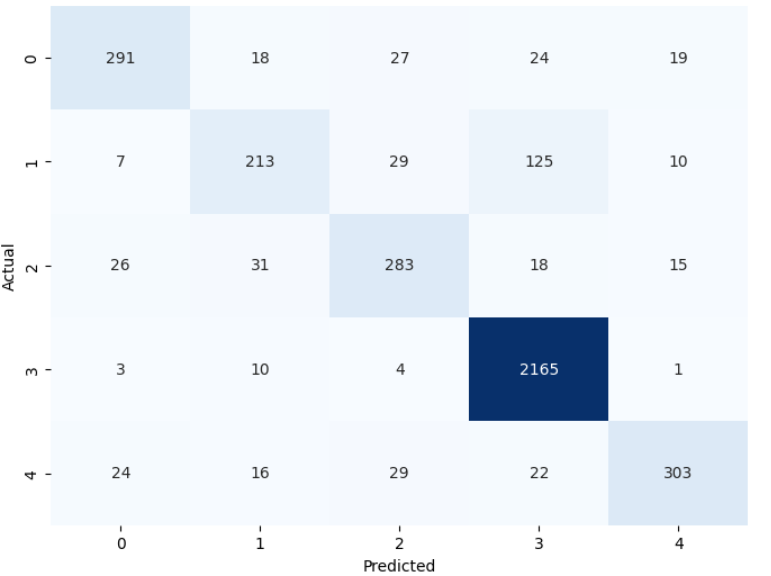
\includegraphics[width=\textwidth]{Images/LR Confusion Matrix.png}
        \caption{Confusion Matrix (Logistic Regression)}
        \label{LRCM}  % Label for referencing the subfigure
    \end{subfigure}
    \hfill
    \begin{subfigure}[b]{0.49\textwidth}
        \centering
        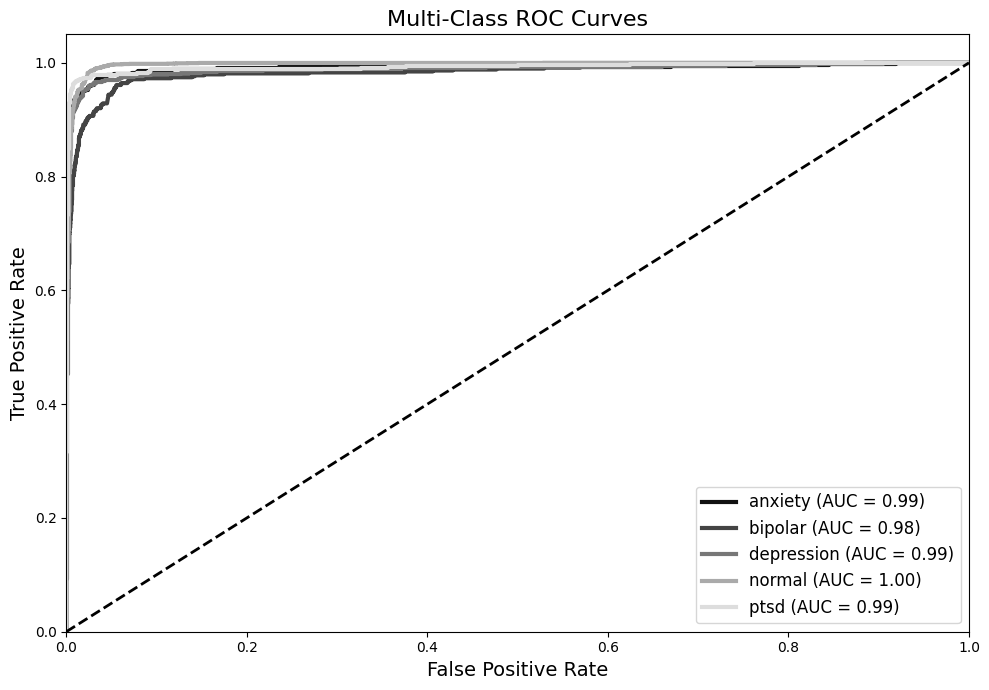
\includegraphics[width=\textwidth]{Images/LR ROC.png}
        \caption{ROC AUC (Logistic Regression)}
        \label{LRROC}  % Label for referencing the subfigure
    \end{subfigure}
    \caption{Evaluation Results for Logistic Regression}
    \label{fig:comparison}
\end{figure}

\pagebreak
% --------- naive bayes

\subsection{Results of Naive Bayes}

\begin{center}
    \textbf{Naive Bayes Classification Report} \\[0.5em]
    \begin{tabular}{|l|c|c|c|c|}
        \hline
        \textbf{Class} & \textbf{Precision} & \textbf{Recall} & \textbf{F1-Score} & \textbf{Support} \\ \hline
        Anxiety        & 0.70               & 0.73            & 0.72              & 379              \\ \hline
        Bipolar        & 0.83               & 0.45            & 0.58              & 384              \\ \hline
        Depression     & 0.59               & 0.87            & 0.70              & 373              \\ \hline
        Normal         & 0.96               & 0.92            & 0.94              & 2183             \\ \hline
        PTSD           & 0.71               & 0.83            & 0.76              & 394              \\ \hline
        \textbf{Accuracy} & \multicolumn{4}{|c|}{83.63\%} \\ \hline
        \textbf{Macro Avg} & 0.76            & 0.76            & 0.74              & 3713             \\ \hline
        \textbf{Weighted Avg} & 0.85         & 0.84            & 0.84              & 3713             \\ \hline
    \end{tabular}
\end{center}

\vspace{0.25em}

\begin{center}
    \textbf{ROC Curve Areas for Each Class} \\[0.5em]
    \begin{tabular}{|l|c|}
        \hline
        \textbf{Class}  & \textbf{ROC AUC} \\ \hline
        Anxiety         & 0.92            \\ \hline
        Bipolar         & 0.89            \\ \hline
        Depression      & 0.94            \\ \hline
        Normal          & 0.99            \\ \hline
        PTSD            & 0.94            \\ \hline
    \end{tabular}
\end{center}

\vspace{0.25em}

\begin{figure}[h!]
    \centering
    \begin{subfigure}[b]{0.49\textwidth}
        \centering
        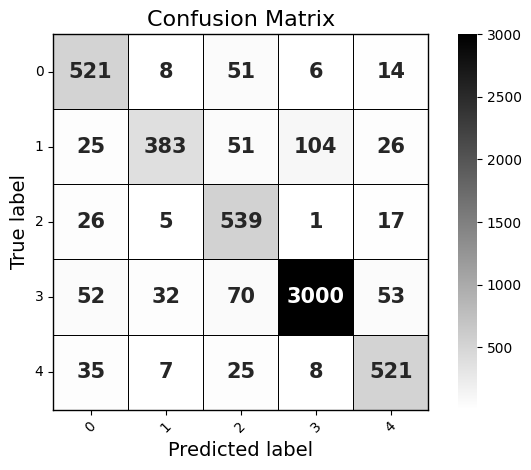
\includegraphics[width=\textwidth]{Images/NB Confusion Matrix.png}
        \caption{Confusion Matrix (Naive Bayes)}
        \label{NBCM}  % Label for referencing the subfigure
    \end{subfigure}
    \hfill
    \begin{subfigure}[b]{0.49\textwidth}
        \centering
        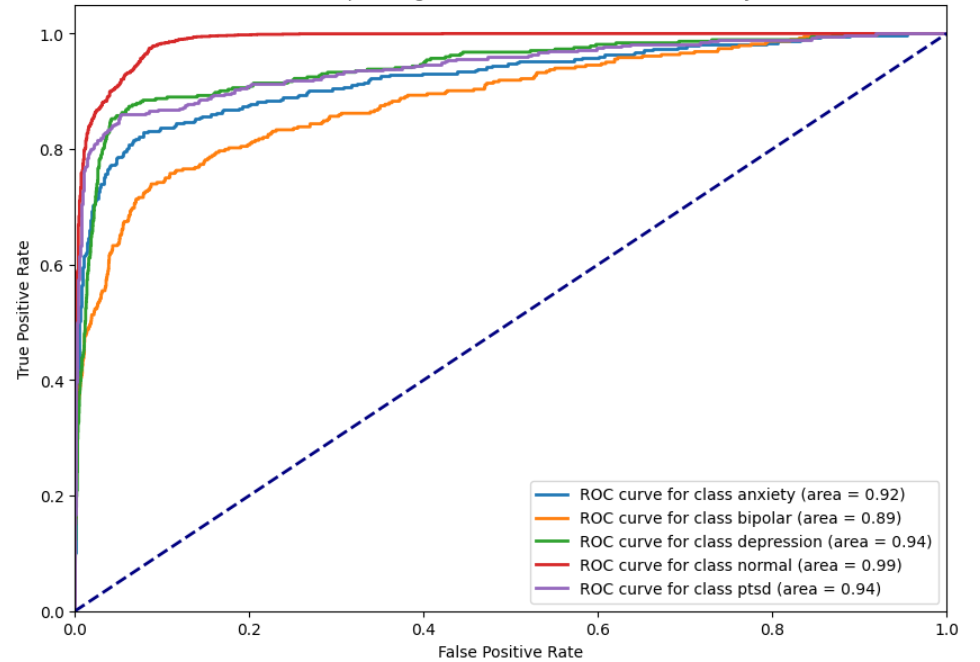
\includegraphics[width=\textwidth]{Images/NB ROC.png}
        \caption{ROC AUC (Naive Bayes)}
        \label{NBROC}  % Label for referencing the subfigure
    \end{subfigure}
    \caption{Evaluation Results for Naive Bayes}
    \label{fig:nb_comparison}
\end{figure}

\pagebreak
% ------------- svc

\subsection{Results of Support Vector Machine}

\begin{center}
    \textbf{SVM Classification Report} \\[0.5em]
    \begin{tabular}{|l|c|c|c|c|}
        \hline
        \textbf{Class} & \textbf{Precision} & \textbf{Recall} & \textbf{F1-Score} & \textbf{Support} \\ \hline
        Anxiety        & 0.72               & 0.76            & 0.74              & 379              \\ \hline
        Bipolar        & 0.62               & 0.61            & 0.61              & 384              \\ \hline
        Depression     & 0.74               & 0.71            & 0.72              & 373              \\ \hline
        Normal         & 0.94               & 0.95            & 0.95              & 2183             \\ \hline
        PTSD           & 0.78               & 0.74            & 0.76              & 394              \\ \hline
        \textbf{Accuracy} & \multicolumn{4}{|c|}{85.13\%} \\ \hline
        \textbf{Macro Avg} & 0.76            & 0.75            & 0.76              & 3713             \\ \hline
        \textbf{Weighted Avg} & 0.85         & 0.85            & 0.85              & 3713             \\ \hline
    \end{tabular}
\end{center}

\vspace{0.25em}

\begin{center}
    \textbf{ROC Curve Areas for Each Class} \\[0.5em]
    \begin{tabular}{|l|c|}
        \hline
        \textbf{Class}  & \textbf{ROC AUC} \\ \hline
        Anxiety         & 0.96            \\ \hline
        Bipolar         & 0.90            \\ \hline
        Depression      & 0.96            \\ \hline
        Normal          & 0.98            \\ \hline
        PTSD            & 0.96            \\ \hline
    \end{tabular}
\end{center}

\vspace{0.25em}

\begin{figure}[h!]
    \centering
    \begin{subfigure}[b]{0.49\textwidth}
        \centering
        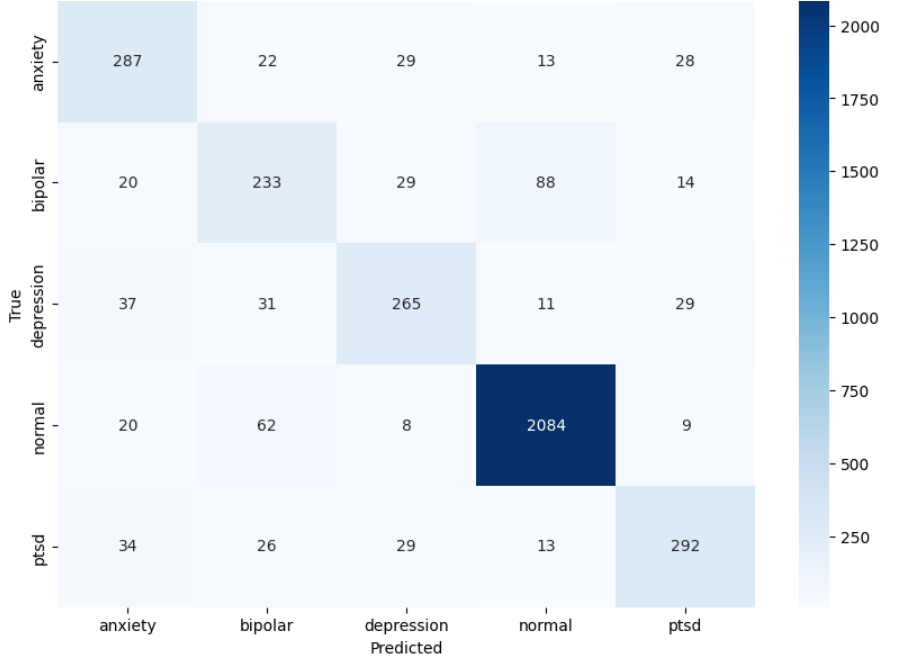
\includegraphics[width=\textwidth]{Images/SVM Confusion Matrix.png}
        \caption{Confusion Matrix (SVM)}
        \label{SVMCM}  % Label for referencing the subfigure
    \end{subfigure}
    \hfill
    \begin{subfigure}[b]{0.49\textwidth}
        \centering
        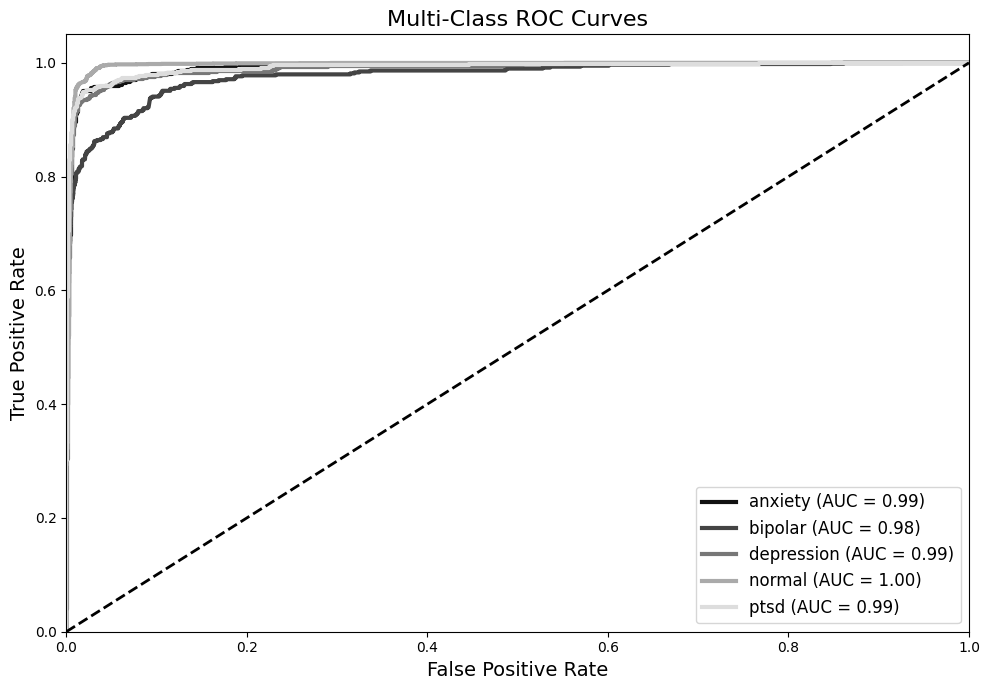
\includegraphics[width=\textwidth]{Images/SVM ROC.png}
        \caption{ROC AUC (SVM)}
        \label{SVMROC}  % Label for referencing the subfigure
    \end{subfigure}
    \caption{Evaluation Results for SVM}
    \label{fig:svm_comparison}
\end{figure}

% ------------- random forest
\pagebreak

\subsection{Results of Random Forest}

\begin{center}
    \textbf{Random Forest Classification Report} \\[0.5em]
    \begin{tabular}{|l|c|c|c|c|}
        \hline
        \textbf{Class} & \textbf{Precision} & \textbf{Recall} & \textbf{F1-Score} & \textbf{Support} \\ \hline
        Anxiety        & 0.81               & 0.70            & 0.75              & 379              \\ \hline
        Bipolar        & 0.93               & 0.47            & 0.62              & 384              \\ \hline
        Depression     & 0.72               & 0.77            & 0.74              & 373              \\ \hline
        Normal         & 0.88               & 1.00            & 0.93              & 2183             \\ \hline
        PTSD           & 0.92               & 0.74            & 0.82              & 394              \\ \hline
        \textbf{Accuracy} & \multicolumn{4}{|c|}{86.00\%} \\ \hline
        \textbf{Macro Avg} & 0.85            & 0.73            & 0.77              & 3713             \\ \hline
        \textbf{Weighted Avg} & 0.86         & 0.86            & 0.85              & 3713             \\ \hline
    \end{tabular}
\end{center}

\vspace{0.25em}

\begin{center}
    \textbf{ROC Curve Areas for Each Class} \\[0.5em]
    \begin{tabular}{|l|c|}
        \hline
        \textbf{Class}  & \textbf{ROC AUC} \\ \hline
        Anxiety         & 0.96            \\ \hline
        Bipolar         & 0.89            \\ \hline
        Depression      & 0.97            \\ \hline
        Normal          & 0.97            \\ \hline
        PTSD            & 0.97            \\ \hline
    \end{tabular}
\end{center}

\vspace{0.25em}

\begin{figure}[h!]
    \centering
    \begin{subfigure}[b]{0.49\textwidth}
        \centering
        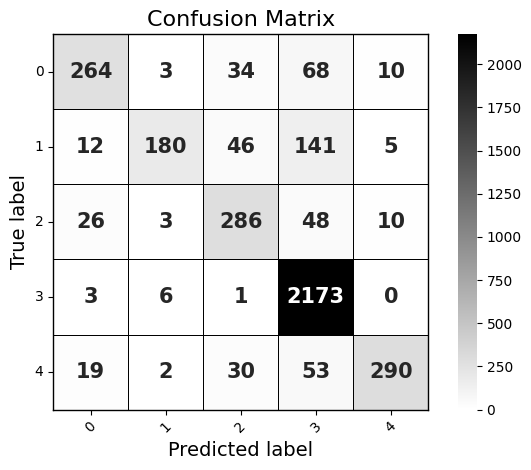
\includegraphics[width=\textwidth]{Images/RF Confusion Matrix.png}
        \caption{Confusion Matrix (Random Forest)}
        \label{RFCM}  % Label for referencing the subfigure
    \end{subfigure}
    \hfill
    \begin{subfigure}[b]{0.49\textwidth}
        \centering
        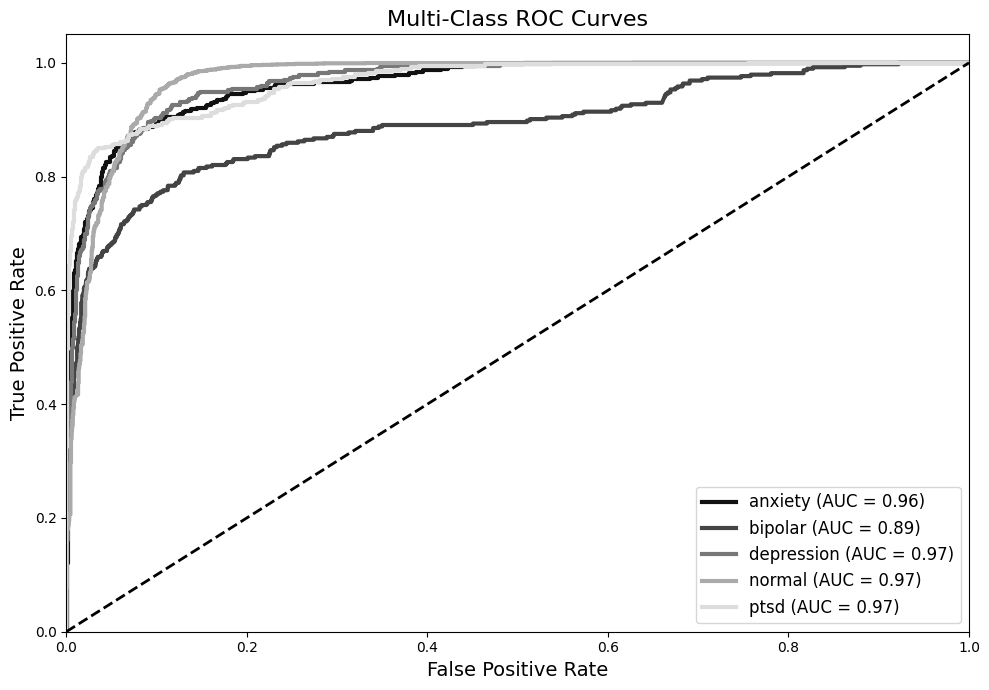
\includegraphics[width=\textwidth]{Images/RF ROC.png}
        \caption{ROC AUC (Random Forest)}
        \label{RFROC}  % Label for referencing the subfigure
    \end{subfigure}
    \caption{Evaluation Results for Random Forest}
    \label{fig:rf_comparison}
\end{figure}

\pagebreak


% -------- xgb

\subsection{Results of XGBoost}

\begin{center}
    \textbf{XGBoost Classification Report} \\[0.5em]
    \begin{tabular}{|l|c|c|c|c|}
        \hline
        \textbf{Class} & \textbf{Precision} & \textbf{Recall} & \textbf{F1-Score} & \textbf{Support} \\ \hline
        Anxiety        & 0.81               & 0.74            & 0.77              & 403              \\ \hline
        Bipolar        & 0.77               & 0.62            & 0.69              & 397              \\ \hline
        Depression     & 0.72               & 0.81            & 0.76              & 387              \\ \hline
        Normal         & 0.93               & 0.98            & 0.95              & 2137             \\ \hline
        PTSD           & 0.86               & 0.75            & 0.80              & 396              \\ \hline
        \textbf{Accuracy} & \multicolumn{4}{|c|}{87.39\%} \\ \hline
        \textbf{Macro Avg} & 0.82            & 0.78            & 0.80              & 3720             \\ \hline
        \textbf{Weighted Avg} & 0.87         & 0.87            & 0.87              & 3720             \\ \hline
    \end{tabular}
\end{center}

\vspace{0.25em}

\begin{center}
    \textbf{ROC Curve Areas for Each Class} \\[0.5em]
    \begin{tabular}{|l|c|}
        \hline
        \textbf{Class}  & \textbf{ROC AUC} \\ \hline
        Anxiety         & 0.97            \\ \hline
        Bipolar         & 0.95            \\ \hline
        Depression      & 0.97            \\ \hline
        Normal          & 0.99            \\ \hline
        PTSD            & 0.97            \\ \hline
    \end{tabular}
\end{center}

\vspace{0.25em}

\begin{figure}[h!]
    \centering
    \begin{subfigure}[b]{0.49\textwidth}
        \centering
        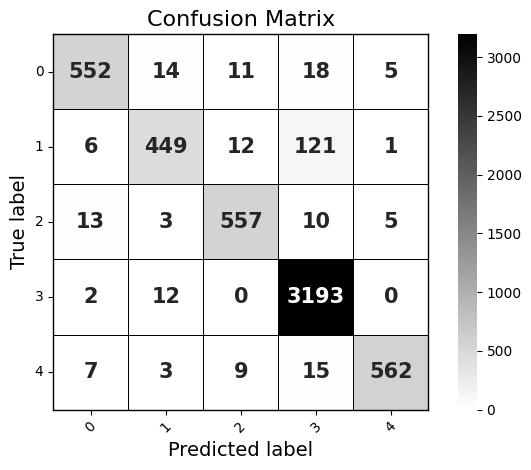
\includegraphics[width=\textwidth]{Images/XG Confusion Matrix.png}
        \caption{Confusion Matrix (XGBoost)}
        \label{XGCM}  % Label for referencing the subfigure
    \end{subfigure}
    \hfill
    \begin{subfigure}[b]{0.49\textwidth}
        \centering
        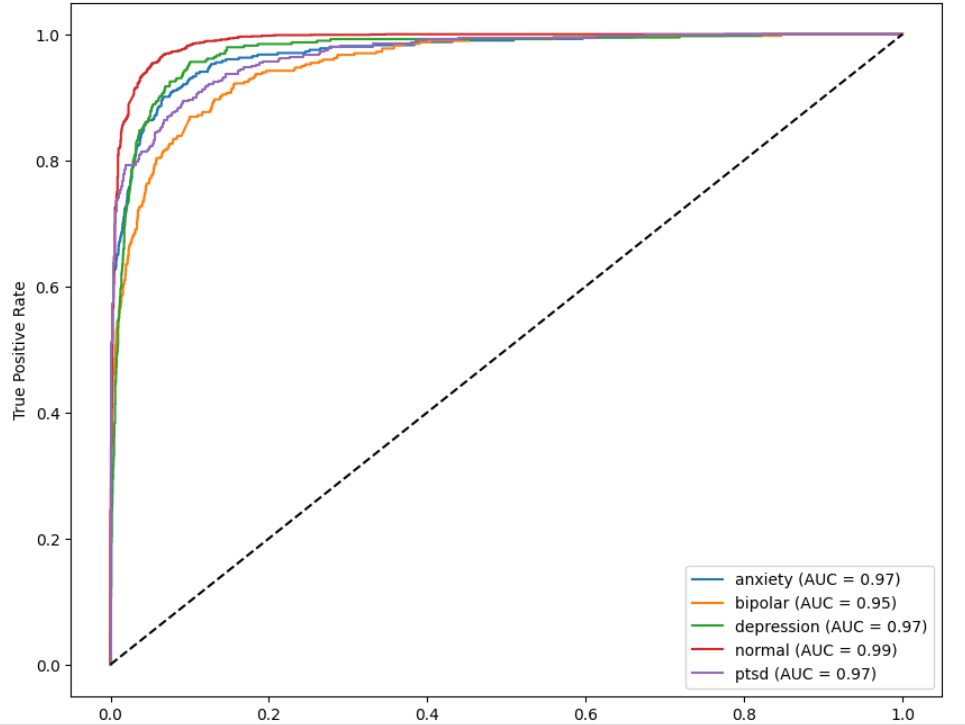
\includegraphics[width=\textwidth]{Images/XG ROC.png}
        \caption{ROC AUC (XGBoost)}
        \label{XGROC}  % Label for referencing the subfigure
    \end{subfigure}
    \caption{Evaluation Results for XGBoost}
    \label{fig:xgboost_comparison}
\end{figure}

\pagebreak

% --------------- knn

\subsection{Results of KNN}

\begin{center}
    \textbf{KNN Classification Report} \\[0.5em]
    \begin{tabular}{|l|c|c|c|c|}
        \hline
        \textbf{Class} & \textbf{Precision} & \textbf{Recall} & \textbf{F1-Score} & \textbf{Support} \\ \hline
        Anxiety        & 0.58               & 0.31            & 0.40              & 379              \\ \hline
        Bipolar        & 0.18               & 0.59            & 0.28              & 384              \\ \hline
        Depression     & 0.47               & 0.39            & 0.43              & 373              \\ \hline
        Normal         & 0.79               & 0.69            & 0.73              & 2183             \\ \hline
        PTSD           & 0.80               & 0.09            & 0.16              & 394              \\ \hline
        \textbf{Accuracy} & \multicolumn{4}{|c|}{54.46\%} \\ \hline
        \textbf{Macro Avg} & 0.56            & 0.41            & 0.40              & 3713             \\ \hline
        \textbf{Weighted Avg} & 0.67         & 0.54            & 0.56              & 3713             \\ \hline
    \end{tabular}
\end{center}

\vspace{0.25em}

\begin{center}
    \textbf{ROC Curve Areas for Each Class} \\[0.5em]
    \begin{tabular}{|l|c|}
        \hline
        \textbf{Class}  & \textbf{ROC AUC} \\ \hline
        Anxiety         & 0.73            \\ \hline
        Bipolar         & 0.67            \\ \hline
        Depression      & 0.77            \\ \hline
        Normal          & 0.80            \\ \hline
        PTSD            & 0.67            \\ \hline
    \end{tabular}
\end{center}

\vspace{0.25em}

\begin{figure}[h!]
    \centering
    \begin{subfigure}[b]{0.49\textwidth}
        \centering
        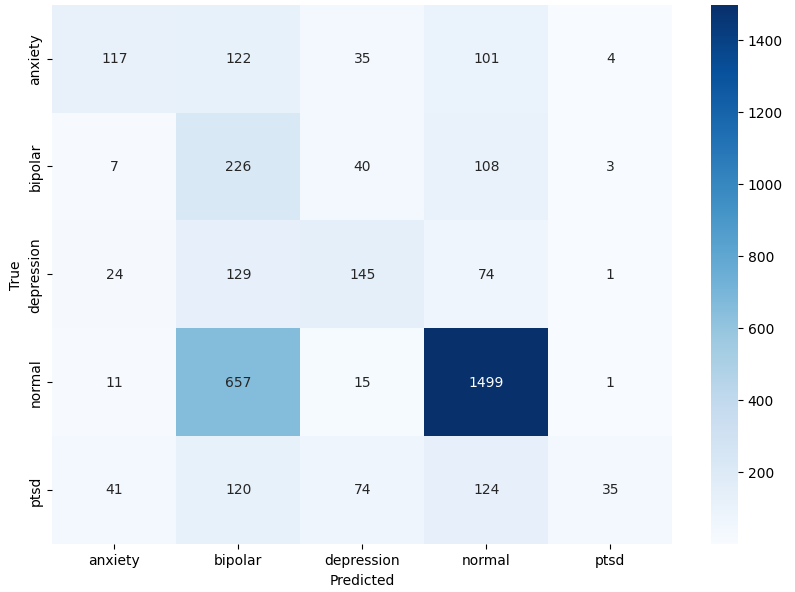
\includegraphics[width=\textwidth]{Images/KNN Confusion Matrix.png}
        \caption{Confusion Matrix (KNN)}
        \label{KNNCM}  % Label for referencing the subfigure
    \end{subfigure}
    \hfill
    \begin{subfigure}[b]{0.49\textwidth}
        \centering
        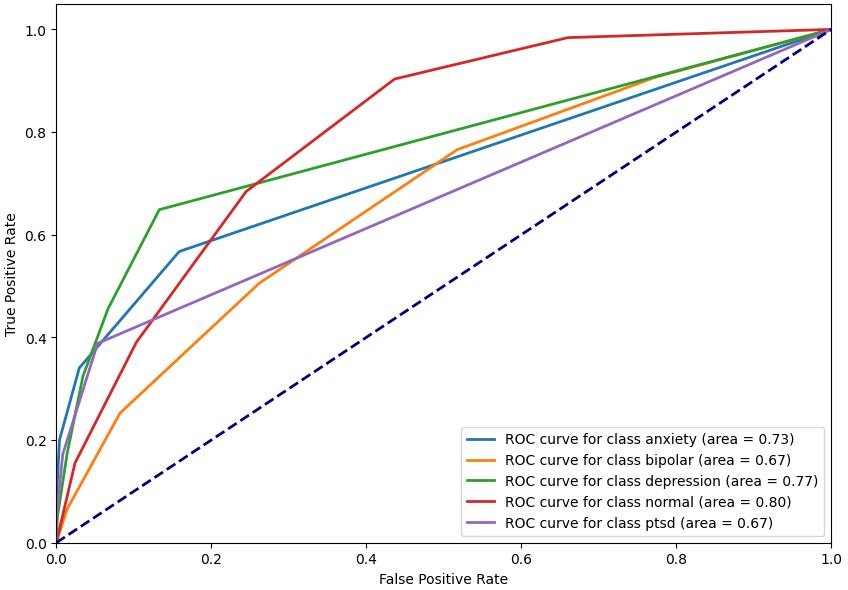
\includegraphics[width=\textwidth]{Images/KNN ROC.png}
        \caption{ROC AUC (KNN)}
        \label{KNNROC}  % Label for referencing the subfigure
    \end{subfigure}
    \caption{Evaluation Results for KNN}
    \label{fig:knn_comparison}
\end{figure}

\pagebreak

% ------ lstm

\subsection{Results of LSTM}

\begin{center}
    \textbf{LSTM Classification Report} \\[0.5em]
    \begin{tabular}{|l|c|c|c|c|}
        \hline
        \textbf{Class} & \textbf{Precision} & \textbf{Recall} & \textbf{F1-Score} & \textbf{Support} \\ \hline
        Anxiety        & 0.74               & 0.72            & 0.73              & 1999             \\ \hline
        Bipolar        & 0.66               & 0.70            & 0.68              & 1964             \\ \hline
        Depression     & 0.68               & 0.69            & 0.69              & 1959             \\ \hline
        Normal         & 0.97               & 0.94            & 0.95              & 10688            \\ \hline
        PTSD           & 0.72               & 0.78            & 0.75              & 1987             \\ \hline
        \textbf{Accuracy} & \multicolumn{4}{|c|}{84.91\%} \\ \hline
        \textbf{Macro Avg} & 0.75            & 0.77            & 0.76              & 18597            \\ \hline
        \textbf{Weighted Avg} & 0.85         & 0.85            & 0.85              & 18597            \\ \hline
    \end{tabular}
\end{center}

\vspace{0.1em}

\begin{center}
    \textbf{ROC Curve Areas for Each Class} \\[0.5em]
    \begin{tabular}{|l|c|}
        \hline
        \textbf{Class}  & \textbf{ROC AUC} \\ \hline
        Anxiety         & 0.95            \\ \hline
        Bipolar         & 0.92            \\ \hline
        Depression      & 0.95            \\ \hline
        Normal          & 0.98            \\ \hline
        PTSD            & 0.95            \\ \hline
    \end{tabular}
\end{center}

\vspace{0.1em}

\begin{figure}[h!]
    \centering
    \begin{subfigure}[b]{0.49\textwidth}
        \centering
        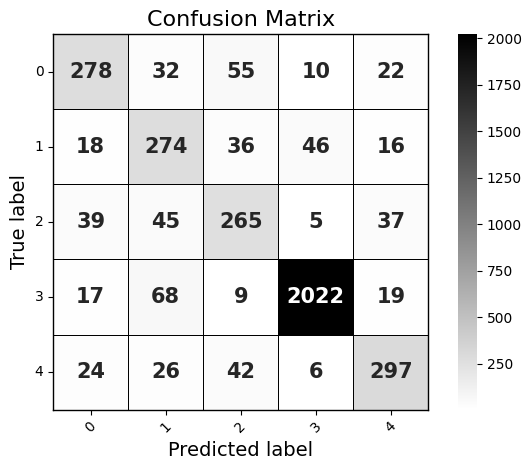
\includegraphics[width=\textwidth]{Images/LSTM Confusion Matrix.png}
        \caption{Confusion Matrix (LSTM)}
        \label{LSTMCM}  % Label for referencing the subfigure
    \end{subfigure}
    \hfill
    \begin{subfigure}[b]{0.49\textwidth}
        \centering
        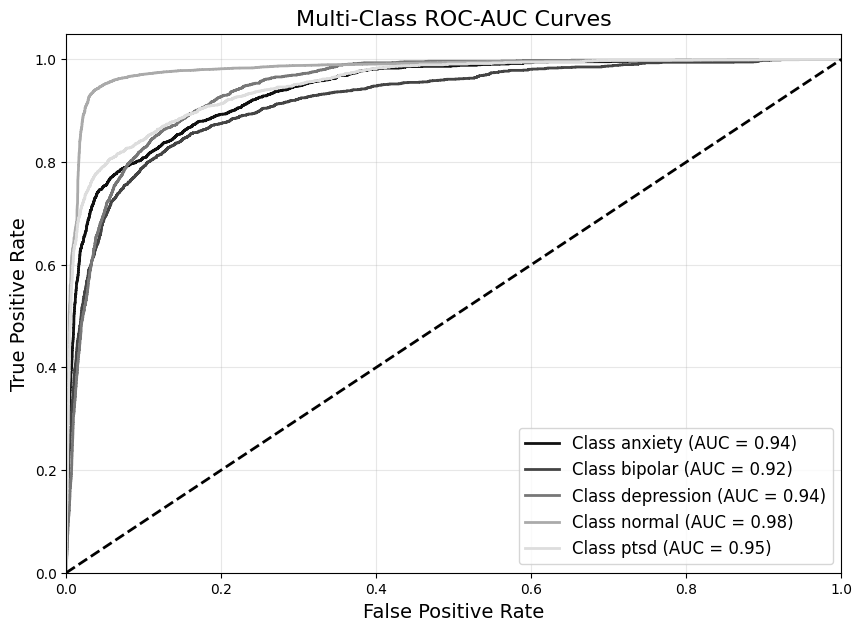
\includegraphics[width=\textwidth]{Images/LSTM ROC.png}
        \caption{ROC AUC (LSTM)}
        \label{LSTMROC}  % Label for referencing the subfigure
    \end{subfigure}
    \caption{Evaluation Results for LSTM}
    \label{fig:lstm_comparison}
\end{figure}

\pagebreak

% -------------- Adding transformer
\subsection{Results from Transformer based model}
\begin{center}
    \textbf{Classification Report} \\[0.5em]
    \begin{tabular}{|l|c|c|c|c|}
        \hline
        \textbf{Class} & \textbf{Precision} & \textbf{Recall} & \textbf{F1-Score} & \textbf{Support} \\ \hline
        Anxiety        & 0.75               & 0.78            & 0.76              & 379             \\ \hline
        Bipolar        & 0.76               & 0.69            & 0.73              & 384             \\ \hline
        Depression     & 0.82               & 0.72            & 0.77              & 373             \\ \hline
        Normal         & 0.95               & 0.97            & 0.96              & 2183            \\ \hline
        PTSD           & 0.79               & 0.80            & 0.79              & 394             \\ \hline
        \textbf{Accuracy} & \multicolumn{4}{|c|}{88.5\%} \\ \hline
        \textbf{Macro Avg} & 0.81            & 0.79            & 0.80              & 3713            \\ \hline
        \textbf{Weighted Avg} & 0.88         & 0.88            & 0.88              & 3713            \\ \hline
    \end{tabular}
\end{center}

\begin{center}
    \textbf{ROC Curve Areas for Each Class} \\[0.5em]
    \begin{tabular}{|l|c|}
        \hline
        \textbf{Class}  & \textbf{ROC AUC} \\ \hline
        Anxiety         & 0.97            \\ \hline
        Bipolar         & 0.94            \\ \hline
        Depression      & 0.98            \\ \hline
        Normal          & 0.99            \\ \hline
        PTSD            & 0.97            \\ \hline
    \end{tabular}
\end{center}

\begin{figure}[h!]
    \centering
    \begin{subfigure}[b]{0.49\textwidth}
        \centering
        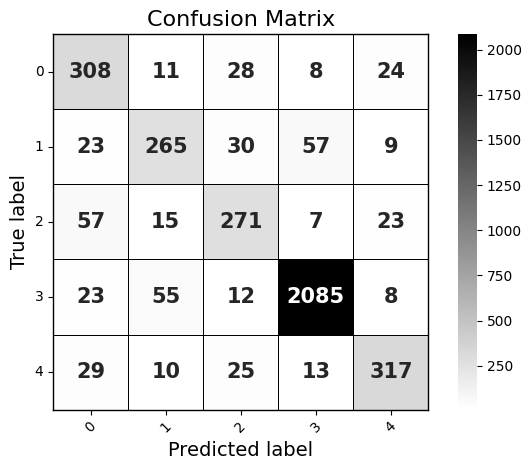
\includegraphics[width=\textwidth]{Images/T CM.png}
        \caption{Confusion Matrix for Transformer based Model}
        \label{dfdl145}  % Label for referencing the subfigure
    \end{subfigure}
    \hfill
    \begin{subfigure}[b]{0.49\textwidth}
        \centering
        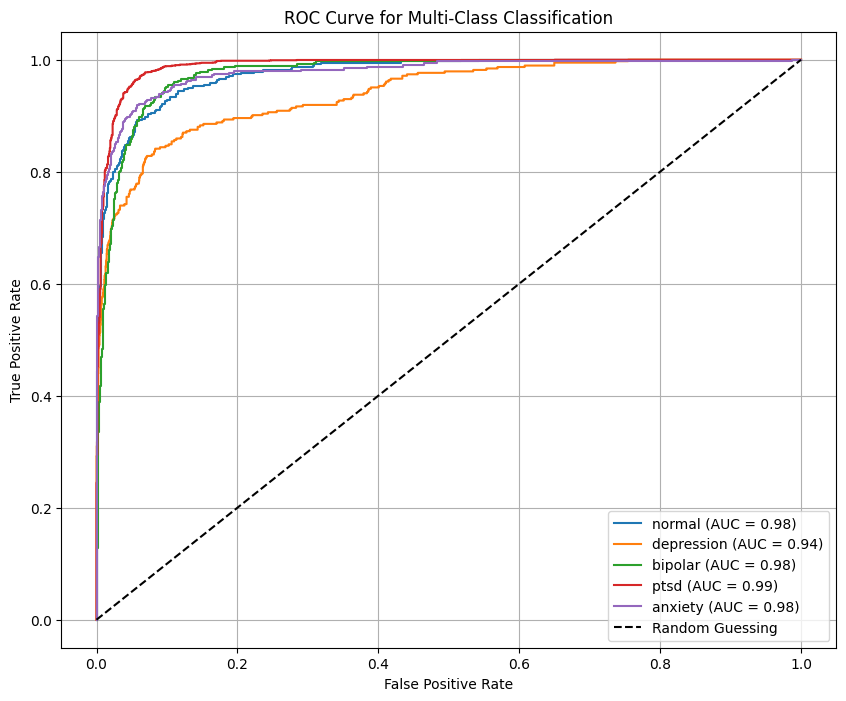
\includegraphics[width=\textwidth]{Images/T ROC.png}
        \caption{ROC AUC for Transformer based Model}
        \label{dfdl146}  % Updated label for referencing the subfigure
    \end{subfigure}
    \caption{Evaluation Results for Transformer based Model}
    \label{fig:transformer_comparison}
\end{figure}


\begin{table}[H]
    \centering
    \renewcommand{\arraystretch}{1.2}
    \small
    \begin{tabularx}{\textwidth}{|l|c|X|}
    \hline
    \textbf{Model} & \textbf{Accuracy (\%)} & \textbf{Key Observations} \\
    \hline
    Logistic Regression & 87.66 & High precision, recall, and F1 for the \textit{Normal} class; struggles with \textit{Bipolar} and \textit{Anxiety}. ROC AUC: Normal (0.99), Anxiety (0.95), Depression (0.96). \\
    \hline
    Naive Bayes & 83.63 & Excellent for \textit{Normal} (Precision 0.96, Recall 0.92, F1 0.94) but poor for \textit{Bipolar} (Recall 0.45, F1 0.58). \newline ROC AUC: Normal (0.99), Depression/PTSD (0.94), Bipolar (0.89). \\
    \hline
    SVM & 85.13 & Best for \textit{Normal} (Precision 0.94, Recall 0.95, F1 0.95); \textit{Bipolar} underperforms (Precision 0.62, Recall 0.61); \textit{Anxiety} is balanced (Recall 0.76, Precision 0.72). \newline ROC AUC: Normal (0.98), others ~0.96, Bipolar (0.90). \\
    \hline
    Random Forest & 86.00 & \textit{Normal} class achieves perfect recall (1.00) with high precision (0.88, F1 0.93); \textit{Bipolar} is weak (Recall 0.47, F1 0.62). \newline ROC AUC: Most classes >0.96; Bipolar (0.89). \\
    \hline
    XGBoost & 87.39 & Strong performance for \textit{Normal}; \textit{Anxiety} shows good metrics (Precision 0.81, Recall 0.74) while \textit{Bipolar} has lower recall (0.62). \newline ROC AUC: 0.97 for Anxiety, Depression, PTSD; 0.99 for Normal. \\
    \hline
    KNN & 54.46 & Overall low performance; \textit{Normal} is moderate (Precision 0.79, Recall 0.69) but \textit{PTSD} has very low recall (0.09). \newline ROC AUC: Normal (0.80), indicating weak discrimination. \\
    \hline
    LSTM & 84.91 & High performance for \textit{Normal}; \textit{Anxiety} acceptable (Precision 0.74, Recall 0.72); \textit{Bipolar} (Precision 0.66, Recall 0.70) and \textit{PTSD} (Precision 0.72, Recall 0.78) are moderate. \newline Effective ROC AUC for Normal. \\
    \hline
    Transformer & 88.50 & Best overall with balanced high precision and recall across all classes. Captures contextual cues effectively and handles class imbalance well. \newline ROC AUC scores range between 0.94 and 0.99. \\
    \hline
    \end{tabularx}
    \caption*{\textbf{Summary Comparison of  Classification Models without Hyperparameter Tuning}}
    \label{tab:model_comparison}
\end{table}


% ----------- hyperparameter tuning

\pagebreak

\subsection{Results of Hyperparameter Tuning}

\noindent
\textbf{Logistic Regression}
\begin{center}
    \textbf{Hyperparameter Tuning on Logistic Regression} \\[0.5em]
    \begin{tabular}{|l|c|}
        \hline
        \textbf{Best Hyperparameters}  & \textbf{Value} \\ \hline
        Solver                        & liblinear      \\ \hline
        Penalty                       & l2             \\ \hline
        C                              & 1              \\ \hline
    \end{tabular}
\end{center}

\begin{center}
    \textbf{Classification Report} \\[0.5em]
    \begin{tabular}{|l|c|c|c|c|}
        \hline
        \textbf{Class} & \textbf{Precision} & \textbf{Recall} & \textbf{F1-Score} & \textbf{Support} \\ \hline
        Anxiety        & 0.83               & 0.77            & 0.80              & 379             \\ \hline
        Bipolar        & 0.74               & 0.55            & 0.64              & 384             \\ \hline
        Depression     & 0.76               & 0.76            & 0.76              & 373             \\ \hline
        Normal         & 0.92               & 0.99            & 0.95              & 2183            \\ \hline
        PTSD           & 0.87               & 0.77            & 0.82              & 394             \\ \hline
        \textbf{Accuracy} & \multicolumn{4}{|c|}{87.72\%} \\ \hline
        \textbf{Macro Avg} & 0.83            & 0.77            & 0.79              & 3713            \\ \hline
        \textbf{Weighted Avg} & 0.87         & 0.88            & 0.87              & 3713            \\ \hline
    \end{tabular}
\end{center}


\begin{center}
    \textbf{ROC Curve Areas for Each Class} \\[0.5em]
    \begin{tabular}{|l|c|}
        \hline
        \textbf{Class}  & \textbf{ROC AUC} \\ \hline
        Anxiety         & 0.95            \\ \hline
        Bipolar         & 0.92            \\ \hline
        Depression      & 0.96            \\ \hline
        Normal          & 0.99            \\ \hline
        PTSD            & 0.95            \\ \hline
    \end{tabular}
\end{center}

\begin{figure}[h!]
    \centering
    \begin{subfigure}[b]{0.49\textwidth}
        \centering
        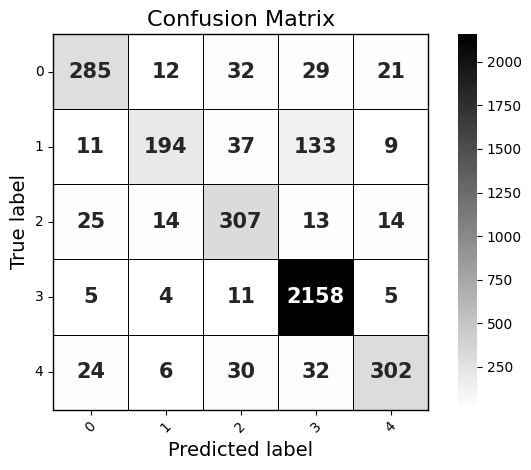
\includegraphics[width=\textwidth]{Images/HP LR CM.png}
        \caption{Classification Matrix after Hyperparameter Tuning (Logistic Regression)}
        \label{LSTMROC2}  % Label for referencing the subfigure
    \end{subfigure}
    \hfill
    \begin{subfigure}[b]{0.49\textwidth}
        \centering
        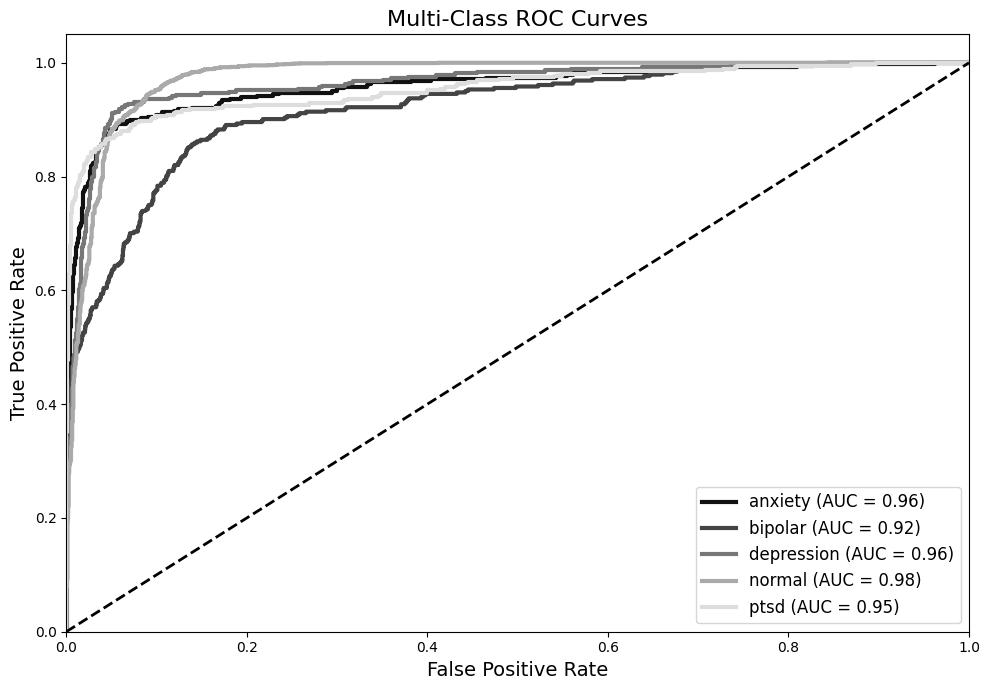
\includegraphics[width=\textwidth]{Images/HP LR ROC.png}
        \caption{ROC AUC after Hyperparameter Tuning (Logistic Regression)}
        \label{LSTMROC3}  % Label for referencing the subfigure
    \end{subfigure}
    \caption{Evaluation Results after Hyperparameter Tuning (Logistic Regression)}
    \label{fig:hp_lr_comparison}
\end{figure}

\pagebreak
% ----------- knn hpt
\vspace{1.5em}
\noindent
\textbf{K-Nearest Neighbours}
\begin{center}
    \textbf{Hyperparameter Tuning on k-NN} \\[0.5em]
    \begin{tabular}{|l|c|}
        \hline
        \textbf{Best Hyperparameters}  & \textbf{Value} \\ \hline
        Weights                       & distance       \\ \hline
        n\_neighbors                  & 10             \\ \hline
        Metric                        & euclidean      \\ \hline
    \end{tabular}
\end{center}

\begin{center}
    \textbf{Classification Report} \\[0.5em]
    \begin{tabular}{|l|c|c|c|c|}
        \hline
        \textbf{Class} & \textbf{Precision} & \textbf{Recall} & \textbf{F1-Score} & \textbf{Support} \\ \hline
        Anxiety        & 0.73               & 0.23            & 0.35              & 379             \\ \hline
        Bipolar        & 0.18               & 0.60            & 0.27              & 384             \\ \hline
        Depression     & 0.47               & 0.40            & 0.43              & 373             \\ \hline
        Normal         & 0.74               & 0.65            & 0.69              & 2183            \\ \hline
        PTSD           & 0.83               & 0.10            & 0.18              & 394             \\ \hline
        \textbf{Accuracy} & \multicolumn{4}{|c|}{52.03\%} \\ \hline
        \textbf{Macro Avg} & 0.59            & 0.40            & 0.39              & 3713            \\ \hline
        \textbf{Weighted Avg} & 0.66         & 0.52            & 0.53              & 3713            \\ \hline
    \end{tabular}
\end{center}

\begin{center}
    \textbf{ROC Curve Areas for Each Class} \\[0.5em]
    \begin{tabular}{|l|c|}
        \hline
        \textbf{Class}  & \textbf{ROC AUC} \\ \hline
        Anxiety         & 0.77            \\ \hline
        Bipolar         & 0.67            \\ \hline
        Depression      & 0.79            \\ \hline
        Normal          & 0.79            \\ \hline
        PTSD            & 0.71            \\ \hline
    \end{tabular}
\end{center}

\begin{figure}[h!]
    \centering
    \begin{subfigure}[b]{0.49\textwidth}
        \centering
        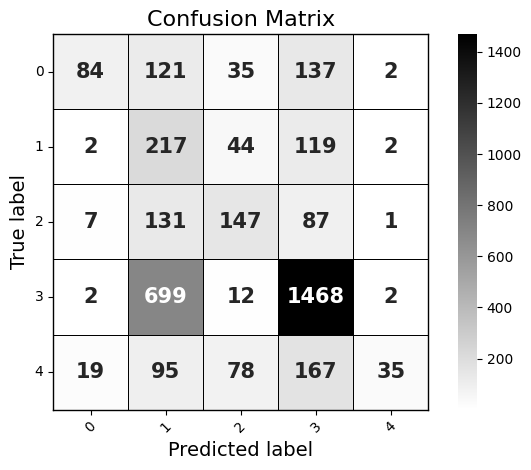
\includegraphics[width=\textwidth]{Images/HP KNN CM.png}
        \caption{Classification Matrix after Hyperparameter Tuning (KNN)}
        \label{LSTMROC4}  % Label for referencing the subfigure
    \end{subfigure}
    \hfill
    \begin{subfigure}[b]{0.49\textwidth}
        \centering
        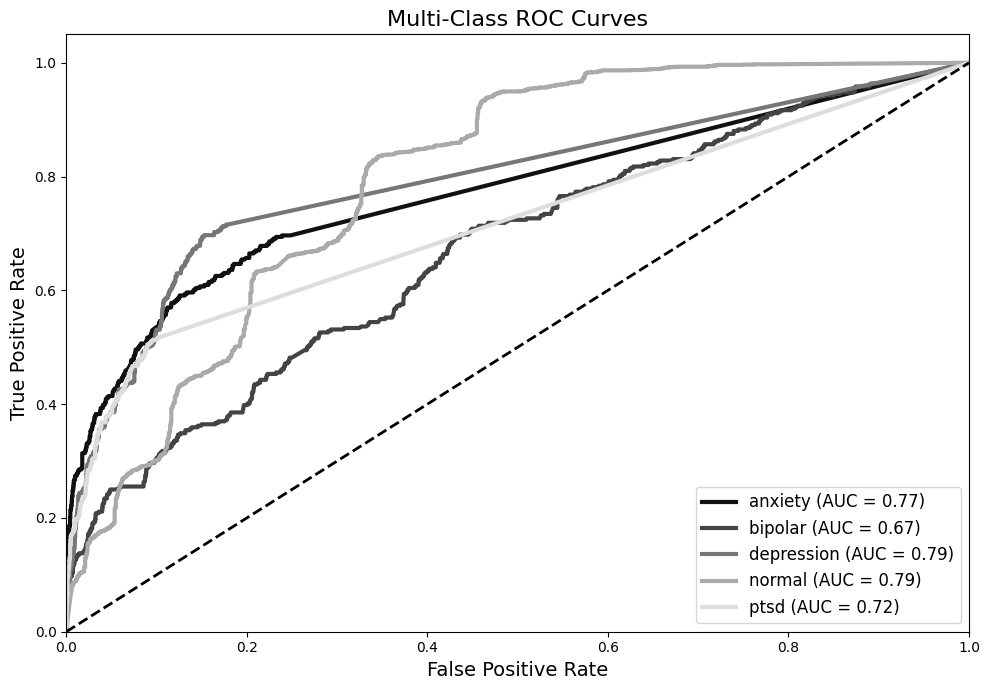
\includegraphics[width=\textwidth]{Images/HP KNN ROC.png}
        \caption{ROC AUC after Hyperparameter Tuning (KNN)}
        \label{LSTMROC5}  % Label for referencing the subfigure
    \end{subfigure}
    \caption{Evaluation Results after Hyperparameter Tuning (KNN)}
    \label{fig:hp_knn_comparison}
\end{figure}

\pagebreak

\vspace{1.5em}
\noindent
\textbf{Support Vector Machine}
\begin{center}
    \textbf{Hyperparameter Tuning on SVM} \\[0.5em]
    \begin{tabular}{|l|c|}
        \hline
        \textbf{Best Hyperparameters}  & \textbf{Value} \\ \hline
        Kernel                        & linear         \\ \hline
        Gamma                         & scale          \\ \hline
        C                              & 1              \\ \hline
    \end{tabular}
\end{center}

\begin{center}
    \textbf{Classification Report} \\[0.5em]
    \begin{tabular}{|l|c|c|c|c|}
        \hline
        \textbf{Class} & \textbf{Precision} & \textbf{Recall} & \textbf{F1-Score} & \textbf{Support} \\ \hline
        Anxiety        & 0.72               & 0.76            & 0.74              & 379             \\ \hline
        Bipolar        & 0.62               & 0.61            & 0.61              & 384             \\ \hline
        Depression     & 0.74               & 0.71            & 0.72              & 373             \\ \hline
        Normal         & 0.94               & 0.95            & 0.95              & 2183            \\ \hline
        PTSD           & 0.78               & 0.74            & 0.76              & 394             \\ \hline
        \textbf{Accuracy} & \multicolumn{4}{|c|}{85.13\%} \\ \hline
        \textbf{Macro Avg} & 0.76            & 0.75            & 0.76              & 3713            \\ \hline
        \textbf{Weighted Avg} & 0.85         & 0.85            & 0.85              & 3713            \\ \hline
    \end{tabular}
\end{center}

\begin{center}
    \textbf{ROC Curve Areas for Each Class} \\[0.5em]
    \begin{tabular}{|l|c|}
        \hline
        \textbf{Class}  & \textbf{ROC AUC} \\ \hline
        Anxiety         & 0.92            \\ \hline
        Bipolar         & 0.88            \\ \hline
        Depression      & 0.95            \\ \hline
        Normal          & 0.98            \\ \hline
        PTSD            & 0.94            \\ \hline
    \end{tabular}
\end{center}

\begin{figure}[h!]
    \centering
    \begin{subfigure}[b]{0.49\textwidth}
        \centering
        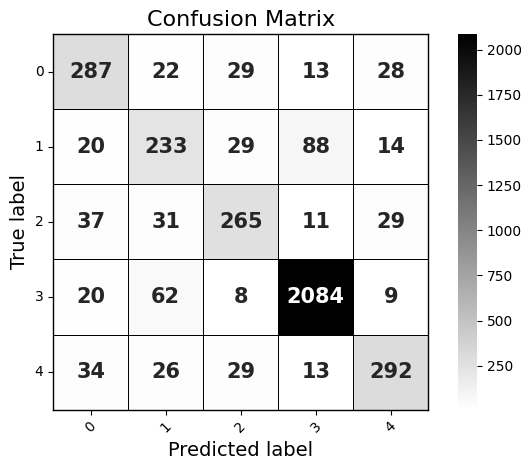
\includegraphics[width=\textwidth]{Images/HP SVM CM.png}
        \caption{Classification Matrix after Hyperparameter Tuning (SVM)}
        \label{LSTMROC6}  % Label for referencing the subfigure
    \end{subfigure}
    \hfill
    \begin{subfigure}[b]{0.49\textwidth}
        \centering
        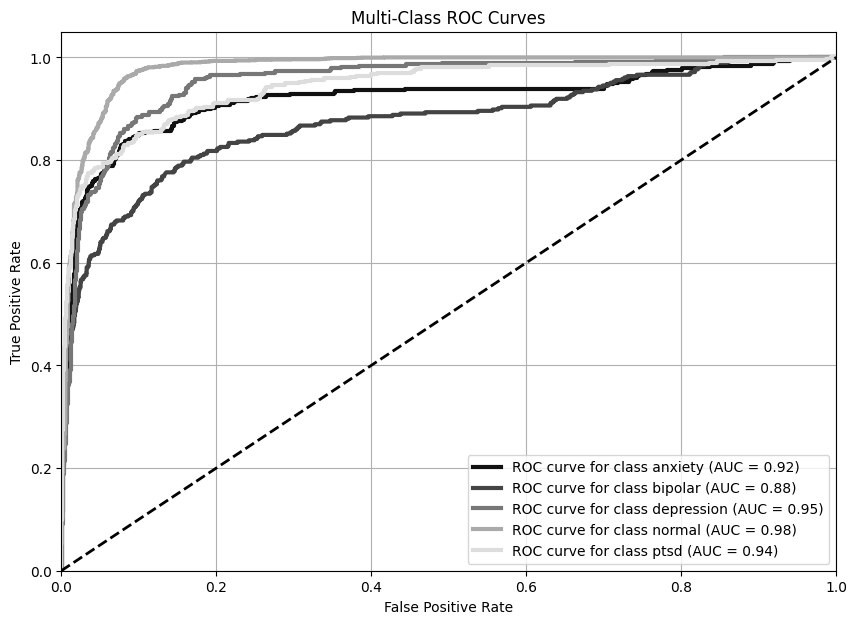
\includegraphics[width=\textwidth]{Images/HP SVM ROC.png}
        \caption{ROC AUC after Hyperparameter Tuning (SVM)}
        \label{LSTMROC}  % Label for referencing the subfigure
    \end{subfigure}
    \caption{Evaluation Results after Hyperparameter Tuning (SVM)}
    \label{fig:hp_svm_comparison}
\end{figure}

\pagebreak


\vspace{1.5em}
\noindent
\textbf{Naive Bayes}
\begin{center}
    \textbf{Hyperparameter Tuning on Naive Bayes} \\[0.5em]
    \begin{tabular}{|l|c|}
        \hline
        \textbf{Best Hyperparameters}  & \textbf{Value} \\ \hline
        Alpha                         & 0.2914180608409973 \\ \hline
    \end{tabular}
\end{center}

\begin{center}
    \textbf{Classification Report} \\[0.5em]
    \begin{tabular}{|l|c|c|c|c|}
        \hline
        \textbf{Class} & \textbf{Precision} & \textbf{Recall} & \textbf{F1-Score} & \textbf{Support} \\ \hline
        Anxiety        & 0.69               & 0.76            & 0.72              & 379             \\ \hline
        Bipolar        & 0.75               & 0.55            & 0.64              & 384             \\ \hline
        Depression     & 0.60               & 0.83            & 0.70              & 373             \\ \hline
        Normal         & 0.96               & 0.91            & 0.94              & 2183            \\ \hline
        PTSD           & 0.73               & 0.79            & 0.76              & 394             \\ \hline
        \textbf{Accuracy} & \multicolumn{4}{|c|}{83.95\%} \\ \hline
        \textbf{Macro Avg} & 0.75            & 0.77            & 0.75              & 3713            \\ \hline
        \textbf{Weighted Avg} & 0.85         & 0.84            & 0.84              & 3713            \\ \hline
    \end{tabular}
\end{center}

\begin{center}
    \textbf{ROC Curve Areas for Each Class} \\[0.5em]
    \begin{tabular}{|l|c|}
        \hline
        \textbf{Class}  & \textbf{ROC AUC} \\ \hline
        Anxiety         & 0.93            \\ \hline
        Bipolar         & 0.93            \\ \hline
        Depression      & 0.93            \\ \hline
        Normal          & 0.99            \\ \hline
        PTSD            & 0.94            \\ \hline
    \end{tabular}
\end{center}

\begin{figure}[h!]
    \centering
    \begin{subfigure}[b]{0.49\textwidth}
        \centering
        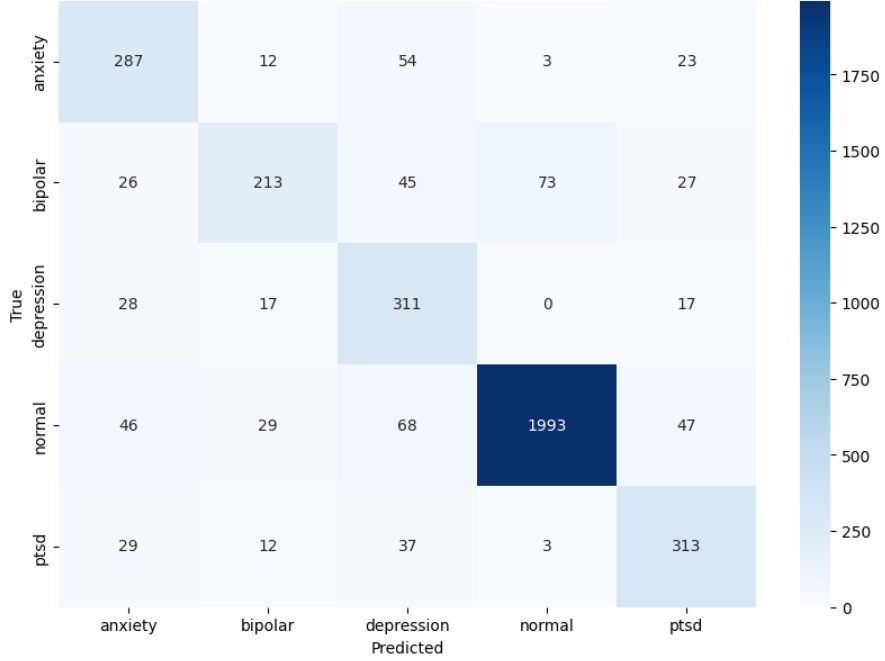
\includegraphics[width=\textwidth]{Images/HP NB CM.png}
        \caption{Classification Matrix after Hyperparameter Tuning (Naive Bayes)}
        \label{LSTMROC7}  % Label for referencing the subfigure
    \end{subfigure}
    \hfill
    \begin{subfigure}[b]{0.49\textwidth}
        \centering
        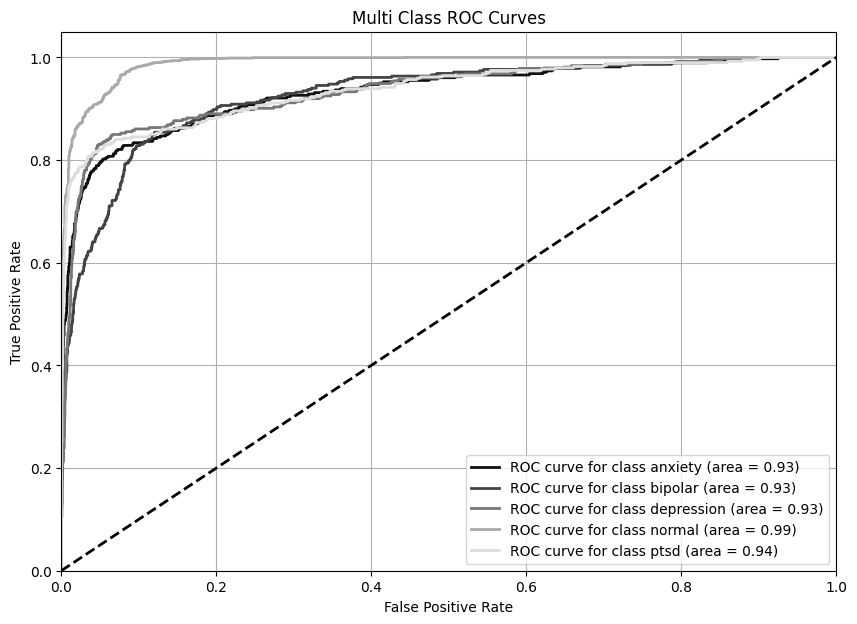
\includegraphics[width=\textwidth]{Images/HP NB ROC.png}
        \caption{ROC AUC after Hyperparameter Tuning (Naive Bayes)}
        \label{LSTMROC8}  % Label for referencing the subfigure
    \end{subfigure}
    \caption{Evaluation Results after Hyperparameter Tuning (Naive Bayes)}
    \label{fig:hp_nb_comparison}
\end{figure}

\pagebreak

\begin{table}[H]
    \centering
    \renewcommand{\arraystretch}{1.3}
    \small
    \begin{tabularx}{\textwidth}{|l|X|X|X|}
        \hline
        \textbf{Model} & \textbf{Best Hyperparameters} & \textbf{Accuracy \& Metrics} & \textbf{Key Observations} \\
        \hline
        Logistic Regression & \texttt{solver=liblinear, penalty=l2, C=1} & Accuracy: 87.72\%; Normal: 92\% accuracy; ROC AUC: Normal 0.99, Depression 0.96 & High precision, recall, and F1 for Normal; Bipolar shows lower F1 (64\%); overall robust performance, especially for Normal and Anxiety. \\
        \hline
        k-NN & \texttt{weights=distance, n\_neighbors=10, metric=euclidean} & Accuracy: 52.03\%; Normal F1: 0.69; ROC AUC: Bipolar 0.67, PTSD 0.71, Normal/Depression 0.79 & Struggles with minority classes: Anxiety (recall 0.23) and PTSD (recall 0.10); not suitable for this dataset. \\
        \hline
        SVM & \texttt{kernel=linear, gamma=scale, C=1} & Accuracy: 85.13\%; F1-scores: Normal 0.95, Depression 0.72, Anxiety 0.74, Bipolar 0.61; ROC AUC: Normal 0.98, Others >0.90, Bipolar 0.90 & Solid overall performance; excellent for Normal and Anxiety, but slightly lower performance for Bipolar. \\
        \hline
        Naive Bayes & \texttt{alpha=0.2914} & Accuracy: 83.95\%; F1-scores: Normal 0.94, PTSD 0.76, Anxiety 0.72; ROC AUC: Normal 0.99, Others >0.90 & Performs very well for Normal and PTSD; lower scores for Bipolar and Depression. \\
        \hline
    \end{tabularx}
    \caption*{\textbf{Summary Comparison of Models after Hyperparameter Tuning}}
    \label{tab:hp_tuning_summary}
\end{table}

\vspace{1em}

\noindent
K-Nearest Neighbors (KNN) performs poorly on this mental health dataset compared to other algorithms, even after hyperparameter tuning. KNN relies on distance-based metrics, which struggle with the sparse, high-dimensional nature of text data, making it difficult to capture meaningful relationships between Reddit posts and mental health labels. Despite optimizing parameters like \verb|weights='distance'|, \verb|n_neighbors=10|, and \verb|metric='euclidean'|, KNN's performance remains suboptimal, with lower accuracy, precision, recall, and F1-score than Logistic Regression, Naive Bayes, or SVM. Its inability to handle non-linear, context-dependent patterns in text, especially for nuanced categories like anxiety, PTSD, or bipolar disorder, highlights its limitations in text classification tasks. KNN's reliance on proximity without considering textual context likely explains its poor performance.

\pagebreak

\begin{figure}[h!]  
    \centering
    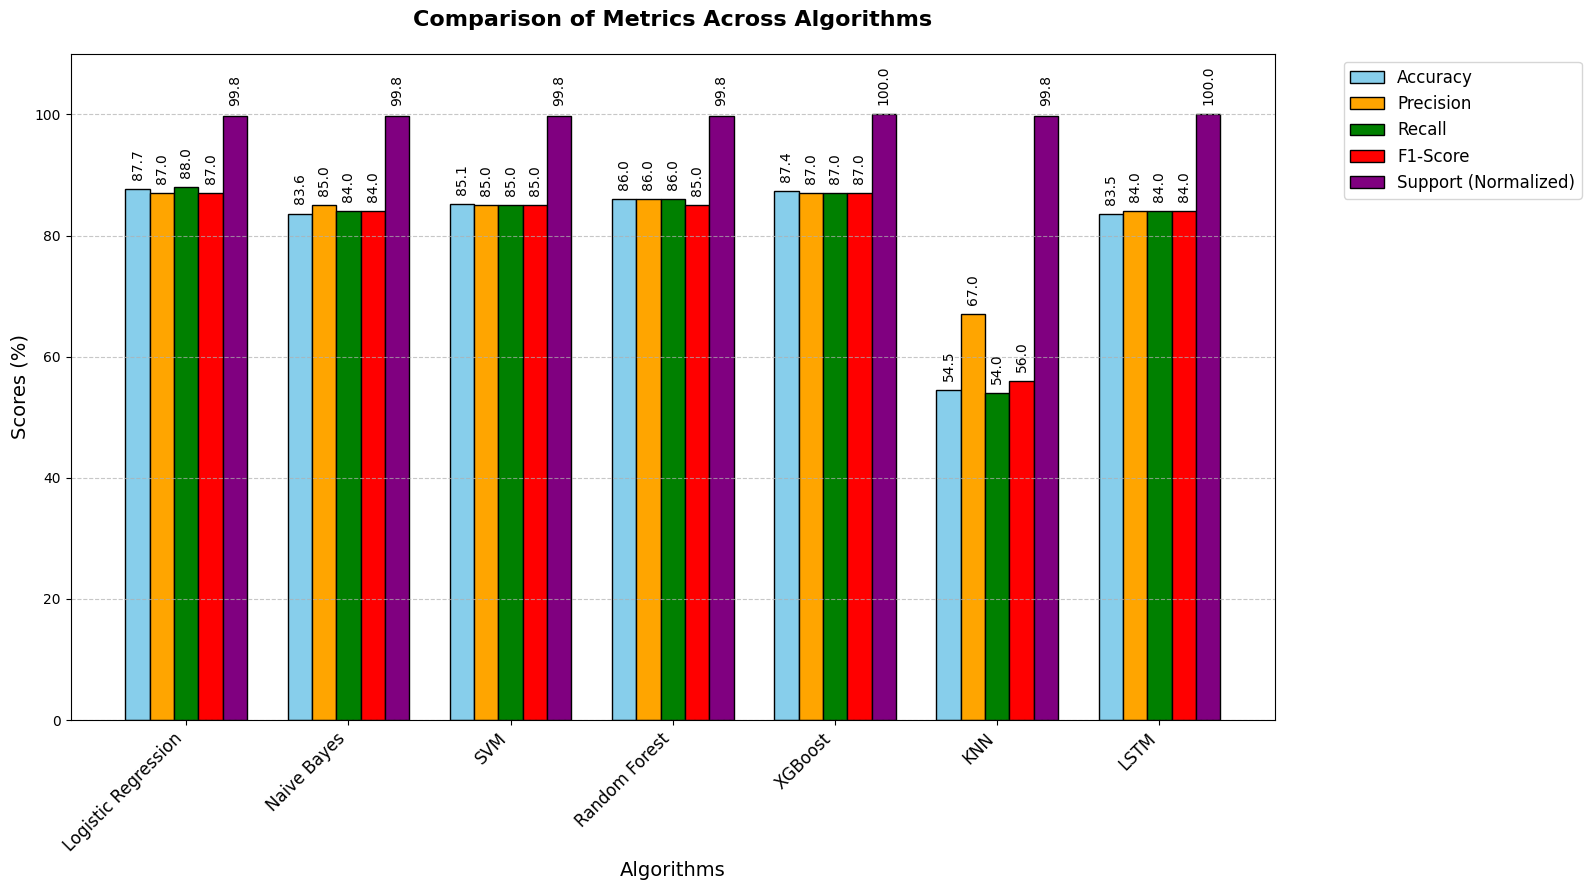
\includegraphics[width=1.0\textwidth]{Images/ML GRAPH 1.png}  
    \caption{Result Comparison of the Algorithms}
    \label{dfdl145}  % Label for referencing the figure
\end{figure}

\begin{figure}[h!]  
    \centering
    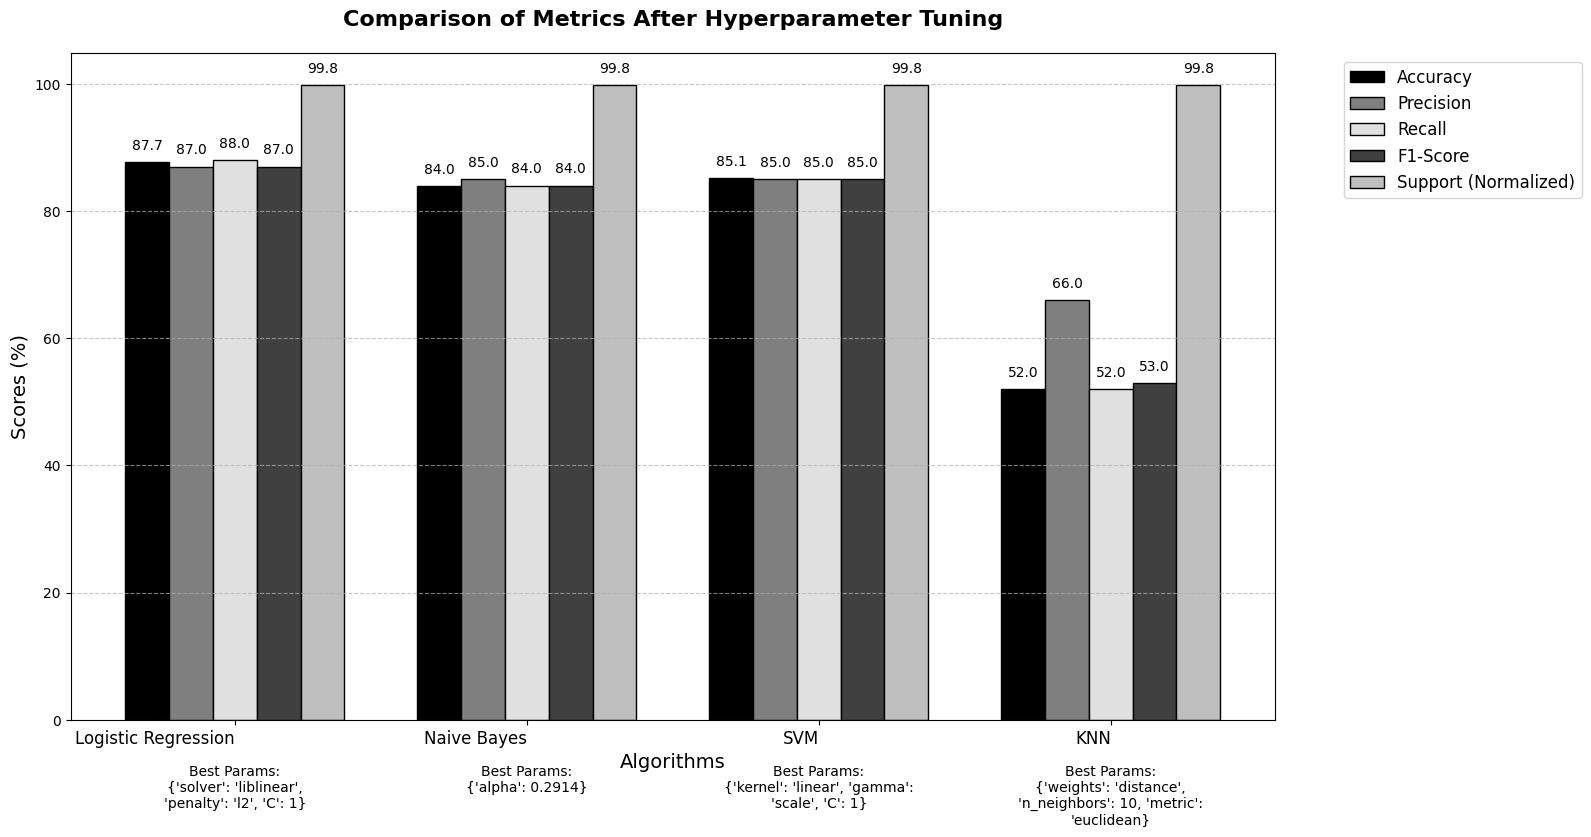
\includegraphics[width=1.0\textwidth]{Images/ML GRAPH 2 HT.png}  
    \caption{Result Comparison after Hyperparameter Tuning}
    \label{dfdl123}  % Label for referencing the figure
\end{figure}

\pagebreak

% ------------------ Different Vectorization ---------
\subsection{Comparison of different tokenizations}
\begin{center}
    \textbf{Model Performance Comparison} \\[0.5em]
    \begin{tabular}{|c|c|c|c|c|c|}
        \hline
        \textbf{Model} & \textbf{BoW} & \textbf{TFIDF} & \textbf{LIWC} & \textbf{Word2Vec} & \textbf{N-Gram} \\ \hline
        \textbf{Logistic Regression} & 87.66 & 86.02 & 66.36 & 79.40 & 87.13 \\ \hline
        \textbf{KNN} & 54.56 & 75.06 & 70.70 & 75.52 & 43.06 \\ \hline
        \textbf{SVC} & 85.13 & 88.26 & 68.14 & 77.89 & 84.33 \\ \hline
        \textbf{Naive Bayes} & 83.63 & 79.42 & 59.63 & 60.44 & 81.71 \\ \hline
        \textbf{Random Forest} & 85.32 & 85.73 & 76.73 & 79.88 & 79.02 \\ \hline
        \textbf{XGB} & 87.42 & 87.39 & 78.56 & 81.01 & 87.96 \\ \hline
    \end{tabular}
\end{center}

\noindent
In ensemble learning, combining models like Logistic Regression (LR), Naive Bayes (NB), K-Nearest Neighbors (KNN), Support Vector Machine (SVM), XGBoost (XGB), Random Forest (RF), and Long Short-Term Memory (LSTM) poses challenges in computational efficiency, model size, and accuracy. Each model has unique strengths and limitations, making their integration complex. LR, NB, and SVM perform well with simpler vectorization methods like Bag of Words (BoW), which efficiently represents text data as sparse vectors. BoW’s simplicity ensures these models remain computationally lightweight while maintaining good classification accuracy. In contrast, XGBoost benefits from more complex feature extraction methods like TFIDF (Term Frequency-Inverse Document Frequency), which captures nuanced relationships by weighting words based on their importance across documents. However, combining TFIDF-based models like XGBoost with BoW-based models can degrade ensemble performance, as the feature representations may not align well. KNN is excluded due to its computational intensity, as it requires storing the entire training dataset and performs poorly with large, high-dimensional datasets. Similarly, Random Forest is omitted because its multiple decision trees increase model size and inference time, outweighing its individual performance benefits. XGBoost, while highly accurate with N-Gram features, is computationally expensive and impractical for real-time systems or large-scale deployment. The choice of feature extraction methods—BoW for LR, NB, and SVM, and TFIDF for XGBoost—balances simplicity and complexity. BoW ensures efficient, interpretable representations for simpler models, while TFIDF provides richer, context-aware features for XGBoost. This combination leverages the strengths of both methods, ensuring each model operates effectively without excessive computational strain. Ultimately, this approach strikes a balance between accuracy and efficiency, enabling the ensemble to perform well while remaining scalable and practical for real-world applications.
\pagebreak

\subsection{Results from Ensemble Model Training and Testing}

\vspace{1em}
\noindent
\textbf{Ensemble Model 1}

\begin{center}
    \textbf{Cross-Validation Accuracy Scores} \\[0.5em]
    \begin{tabular}{|c|c|}
        \hline
        \textbf{Cross-Validation Accuracy Scores} & \textbf{Value} \\ \hline
        1 & 0.96364126 \\ \hline
        2 & 0.95744681 \\ \hline
        3 & 0.96175599 \\ \hline
        4 & 0.95933208 \\ \hline
        5 & 0.96202532 \\ \hline
        \textbf{Mean Validation Accuracy} & \textbf{96.08\%} \\ \hline
    \end{tabular}
\end{center}


\begin{center}
    \textbf{Classification Report for Ensemble Model1} \\[0.5em]
    \begin{tabular}{|c|c|c|c|c|}
        \hline
        & \textbf{Precision} & \textbf{Recall} & \textbf{F1-Score} & \textbf{Support} \\ \hline
        \textbf{Anxiety}    & 0.97 & 0.94 & 0.95 & 400  \\ \hline
        \textbf{Bipolar}    & 0.92 & 0.85 & 0.88 & 388  \\ \hline
        \textbf{Depression} & 0.95 & 0.94 & 0.94 & 392  \\ \hline
        \textbf{Normal}     & 0.97 & 0.99 & 0.98 & 2136 \\ \hline
        \textbf{PTSD}       & 0.97 & 0.96 & 0.96 & 397  \\ \hline
        \textbf{Accuracy}   & \multicolumn{4}{|c|}{\textbf{96.08\%}} \\ \hline
        \textbf{Macro avg}  & 0.96 & 0.93 & 0.95 & 3713 \\ \hline
        \textbf{Weighted avg} & 0.96 & 0.96 & 0.96 & 3713 \\ \hline
    \end{tabular}
\end{center}

\begin{figure}[h!]
    \centering
    \begin{subfigure}[b]{0.49\textwidth}
        \centering
        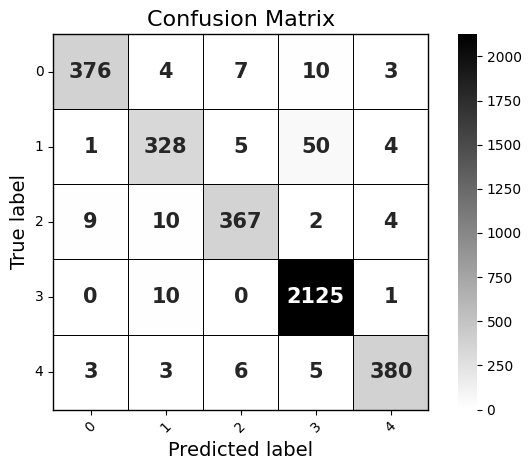
\includegraphics[width=\textwidth]{Images/EM CM.png}
        \caption{Confusion Matrix for Ensemble Model 1}
        \label{dfdl3123}  % Label for referencing the subfigure
    \end{subfigure}
    \hfill
    \begin{subfigure}[b]{0.49\textwidth}
        \centering
        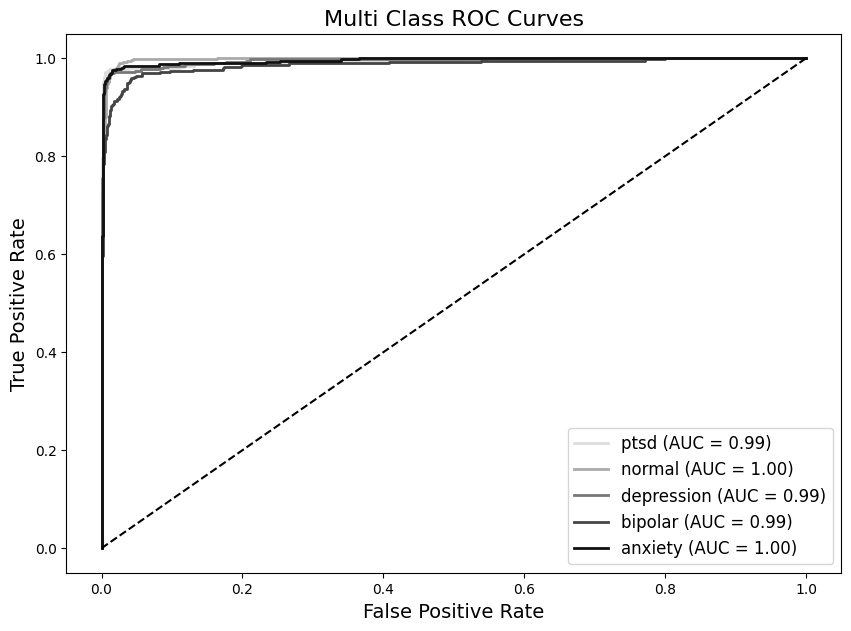
\includegraphics[width=\textwidth]{Images/EM ROC.png}
        \caption{ROC AUC Curve for Ensemble Model 1}
        \label{dfdl12443}  % Label for referencing the subfigure
    \end{subfigure}
    \caption{Evaluation Results for Ensemble Model 1}
    \label{fig:ensemble_model_comparison}
\end{figure}

\pagebreak

\vspace{1em}
\noindent
\textbf{Ensemble Model 2}

\begin{center}
    \textbf{Cross-Validation Accuracy Scores} \\[0.5em]
    \begin{tabular}{|c|c|}
        \hline
        \textbf{Cross-Validation Accuracy Scores} & \textbf{Value} \\ \hline
        1 & 0.980878 \\ \hline
        2 & 0.97629949 \\ \hline
        3 & 0.98249394 \\ \hline
        4 & 0.97522219 \\ \hline
        5 & 0.97710746 \\ \hline
        \textbf{Mean Validation Accuracy} & \textbf{97.84\%} \\ \hline
    \end{tabular}
\end{center}


\begin{center}
    \textbf{Classification Report for Ensemble Model2} \\[0.5em]
    \begin{tabular}{|c|c|c|c|c|}
        \hline
        & \textbf{Precision} & \textbf{Recall} & \textbf{F1-Score} & \textbf{Support} \\ \hline
        \textbf{Anxiety}    & 0.97 & 0.97 & 0.97 & 400  \\ \hline
        \textbf{Bipolar}    & 0.95 & 0.92 & 0.93 & 388  \\ \hline
        \textbf{Depression} & 0.98 & 0.96 & 0.97 & 392  \\ \hline
        \textbf{Normal}     & 0.99 & 0.99 & 0.99 & 2136 \\ \hline
        \textbf{PTSD}       & 0.97 & 0.98 & 0.98 & 397  \\ \hline
        \textbf{Accuracy}   & \multicolumn{4}{|c|}{\textbf{97.93\%}} \\ \hline
        \textbf{Macro avg}  & 0.97 & 0.97 & 0.97 & 3713 \\ \hline
        \textbf{Weighted avg} & 0.98 & 0.98 & 0.98 & 3713 \\ \hline
    \end{tabular}
\end{center}

\begin{figure}[h!]
    \centering
    \begin{subfigure}[b]{0.49\textwidth}
        \centering
        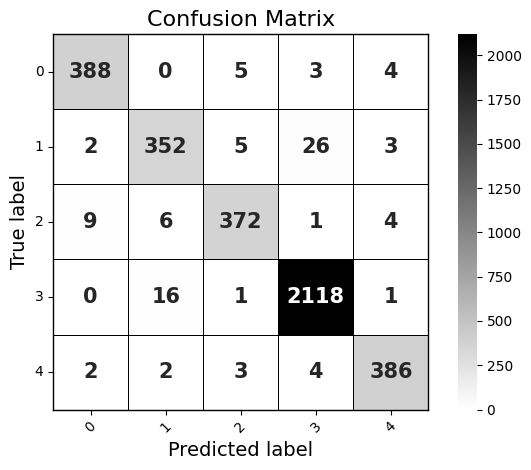
\includegraphics[width=\textwidth]{Images/EM2 CM.png}
        \caption{Confusion Matrix for Ensemble Model 2}
        \label{em2 cm}  % Label for referencing the subfigure
    \end{subfigure}
    \hfill
    \begin{subfigure}[b]{0.49\textwidth}
        \centering
        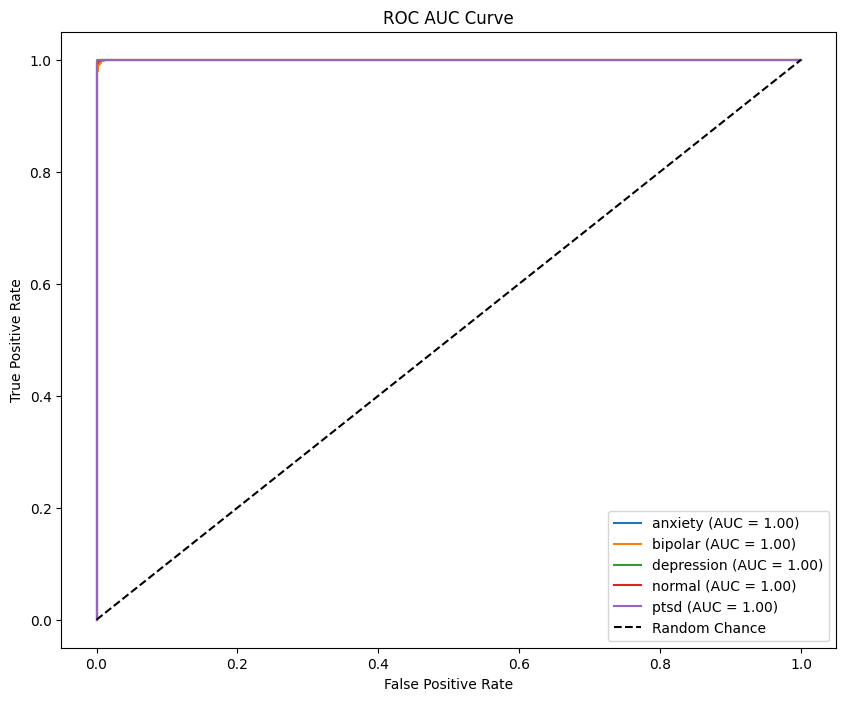
\includegraphics[width=\textwidth]{Images/EM2 ROC.png}
        \caption{ROC AUC for Ensemble Model 2}
        \label{em2 roc}  % Label for referencing the subfigure
    \end{subfigure}
    \caption{Evaluation Results for Ensemble Model 2}
    \label{fig:ensemble_model2_comparison}
\end{figure}

\pagebreak

\noindent
\textbf{Ensemble Model 3}
\begin{center}
    \textbf{Cross-Validation Accuracy Scores} \\[0.5em]
    \begin{tabular}{|c|c|}
        \hline
        \textbf{Cross-Validation Accuracy Scores} & \textbf{Value} \\ \hline
        1 & 0.98195529 \\ \hline
        2 & 0.97549152 \\ \hline
        3 & 0.98060867 \\ \hline
        4 & 0.97603016 \\ \hline
        5 & 0.97629949 \\ \hline
        \textbf{Mean Validation Accuracy} & \textbf{97.81\%} \\ \hline
    \end{tabular}
\end{center}

\begin{center}
    \textbf{Classification Report for Ensemble Model3} \\[0.5em]
    \begin{tabular}{|c|c|c|c|c|}
        \hline
        & \textbf{Precision} & \textbf{Recall} & \textbf{F1-Score} & \textbf{Support} \\ \hline
        \textbf{Anxiety}    & 0.98 & 0.97 & 0.98 & 400  \\ \hline
        \textbf{Bipolar}    & 0.96 & 0.90 & 0.93 & 388  \\ \hline
        \textbf{Depression} & 0.97 & 0.96 & 0.96 & 392  \\ \hline
        \textbf{Normal}     & 0.98 & 1.00 & 0.99 & 2136 \\ \hline
        \textbf{PTSD}       & 0.97 & 0.97 & 0.97 & 397  \\ \hline
        \textbf{Accuracy}   & \multicolumn{4}{|c|}{\textbf{97.76\%}} \\ \hline
        \textbf{Macro avg}  & 0.97 & 0.96 & 0.97 & 3713 \\ \hline
        \textbf{Weighted avg} & 0.98 & 0.98 & 0.98 & 3713 \\ \hline
    \end{tabular}
\end{center}

\begin{figure}[h!]
    \centering
    \begin{subfigure}[b]{0.48\textwidth}
        \centering
        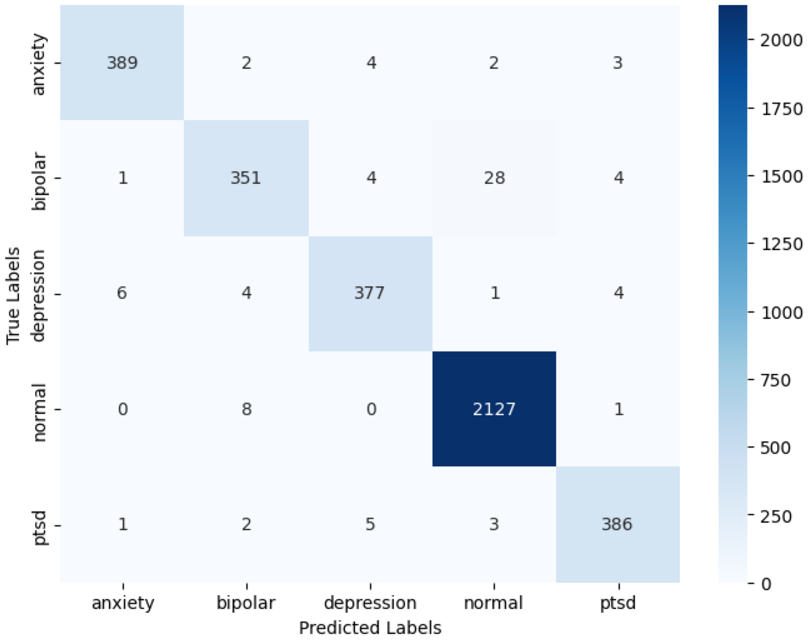
\includegraphics[width=\textwidth]{Images/EM3 CM.png}
        \caption{Confusion Matrix for Ensemble Model 3}
        \label{em3 cm}  % Label for referencing the subfigure
    \end{subfigure}
    \hfill
    \begin{subfigure}[b]{0.48\textwidth}
        \centering
        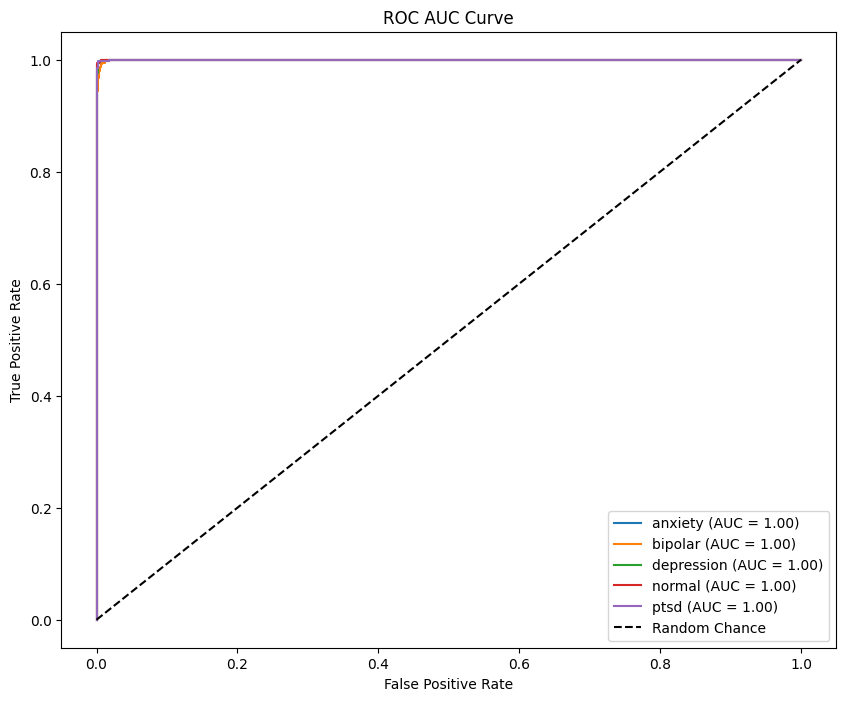
\includegraphics[width=\textwidth]{Images/EM3 ROC.png}
        \caption{ROC AUC for Ensemble Model 3}
        \label{em3 roc}  % Label for referencing the subfigure
    \end{subfigure}
    \caption{Evaluation Results for Ensemble Model 3}
    \label{fig:ensemble_model3_comparison}
\end{figure}

\pagebreak

\vspace{1em}
\noindent
\textbf{Ensemble Model 4}

\begin{center}
    \textbf{Cross-Validation Accuracy Scores} \\[0.5em]
    \begin{tabular}{|c|c|}
        \hline
        \textbf{Cross-Validation Accuracy Scores} & \textbf{Value} \\ \hline
        1 & 0.97683814 \\ \hline
        2 & 0.96821977 \\ \hline
        3 & 0.97872340 \\ \hline
        4 & 0.96821977 \\ \hline
        5 & 0.97225963 \\ \hline
        \textbf{Mean Validation Accuracy} & \textbf{97.29\%} \\ \hline
    \end{tabular}
\end{center}

\begin{center}
    \textbf{Classification Report for Ensemble Model4} \\[0.5em]
    \begin{tabular}{|c|c|c|c|c|}
        \hline
        \textbf{Class} & \textbf{Precision} & \textbf{Recall} & \textbf{F1-Score} & \textbf{Support} \\ \hline
        Anxiety & 0.97 & 0.97 & 0.97 & 400 \\ \hline
        Bipolar & 0.95 & 0.90 & 0.92 & 388 \\ \hline
        Depression & 0.97 & 0.95 & 0.96 & 392 \\ \hline
        Normal & 0.99 & 0.99 & 0.99 & 2136 \\ \hline
        PTSD & 0.97 & 0.98 & 0.97 & 397 \\ \hline
        \textbf{Accuracy} & \multicolumn{4}{c|}{\textbf{97.63\%}} \\ \hline
        \textbf{Macro Avg} & 0.97 & 0.96 & 0.96 & 3713 \\ \hline
        \textbf{Weighted Avg} & 0.98 & 0.98 & 0.98 & 3713 \\ \hline
    \end{tabular}
\end{center}

\begin{figure}[h!]
    \centering
    \begin{subfigure}[b]{0.49\textwidth}
        \centering
        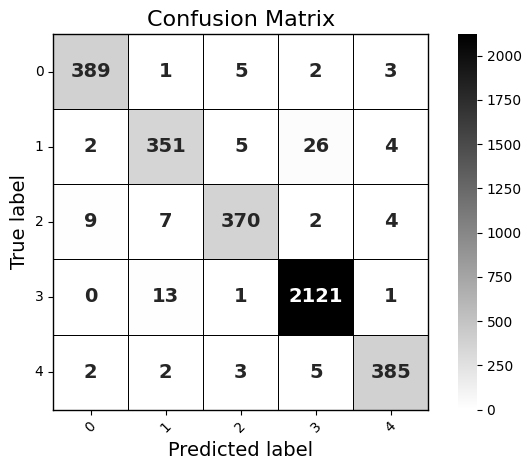
\includegraphics[width=\textwidth]{Images/BAG CM.png}
        \caption{Confusion Matrix for Ensemble Model 4}
        \label{bag cm}  % Label for referencing the subfigure
    \end{subfigure}
    \hfill
    \begin{subfigure}[b]{0.49\textwidth}
        \centering
        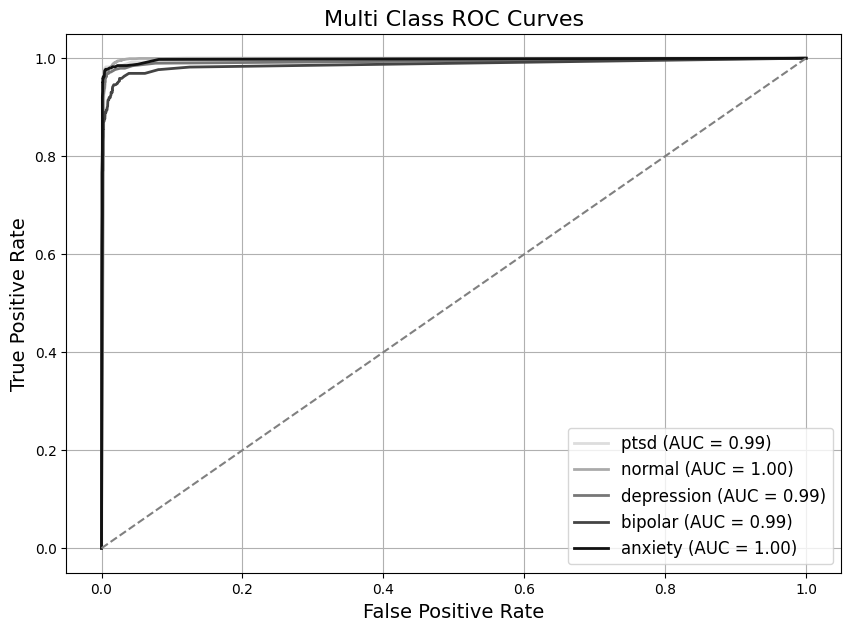
\includegraphics[width=\textwidth]{Images/BAG ROC.png}
        \caption{ROC AUC for Ensemble Model 4}
        \label{bag roc}  % Label for referencing the subfigure
    \end{subfigure}
    \caption{Evaluation Results for Ensemble Model 4}
    \label{fig:ensemble_model4_comparison}
\end{figure}

\pagebreak

\noindent
\textbf{Ensemble Model 5}

\begin{center}
    \textbf{Cross-Validation Accuracy Scores} \\[0.5em]
    \begin{tabular}{|c|c|}
        \hline
        \textbf{Cross-Validation Accuracy Scores} & \textbf{Value} \\ \hline
        1 & 0.96768765 \\ \hline
        2 & 0.97273645 \\ \hline
        3 & 0.97306397 \\ \hline
        4 & 0.96801347 \\ \hline
        5 & 0.96767677 \\ \hline
        \textbf{Mean Validation Accuracy} & \textbf{96.98\%} \\ \hline
    \end{tabular}
\end{center}


\begin{center}
    \textbf{Classification Report for Ensemble Model5} \\[0.5em]
    \begin{tabular}{|c|c|c|c|c|}
        \hline
        & \textbf{Precision} & \textbf{Recall} & \textbf{F1-Score} & \textbf{Support} \\ \hline
        \textbf{Anxiety}    & 0.96 & 0.95 & 0.96 & 400 \\ \hline
        \textbf{Bipolar}    & 0.94 & 0.89 & 0.92 & 388 \\ \hline
        \textbf{Depression} & 0.96 & 0.95 & 0.95 & 392 \\ \hline
        \textbf{Normal}     & 0.98 & 0.99 & 0.99 & 2136 \\ \hline
        \textbf{PTSD}       & 0.97 & 0.97 & 0.97 & 397 \\ \hline
        \textbf{Accuracy}   & \multicolumn{4}{c|}{\textbf{97.17\%}} \\ \hline
        \textbf{Macro avg}  & 0.96 & 0.95 & 0.96 & 3713 \\ \hline
        \textbf{Weighted avg} & 0.97 & 0.97 & 0.97 & 3713 \\ \hline
    \end{tabular}
\end{center}

\begin{figure}[h!]
    \centering
    \begin{subfigure}[b]{0.49\textwidth}
        \centering
        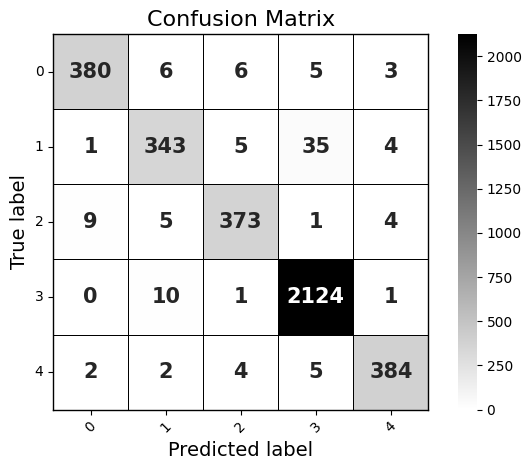
\includegraphics[width=\textwidth]{Images/BLD CM.png}
        \caption{Confusion Matrix for Ensemble Model 5}
        \label{bld cm}  % Label for referencing the subfigure
    \end{subfigure}
    \hfill
    \begin{subfigure}[b]{0.49\textwidth}
        \centering
        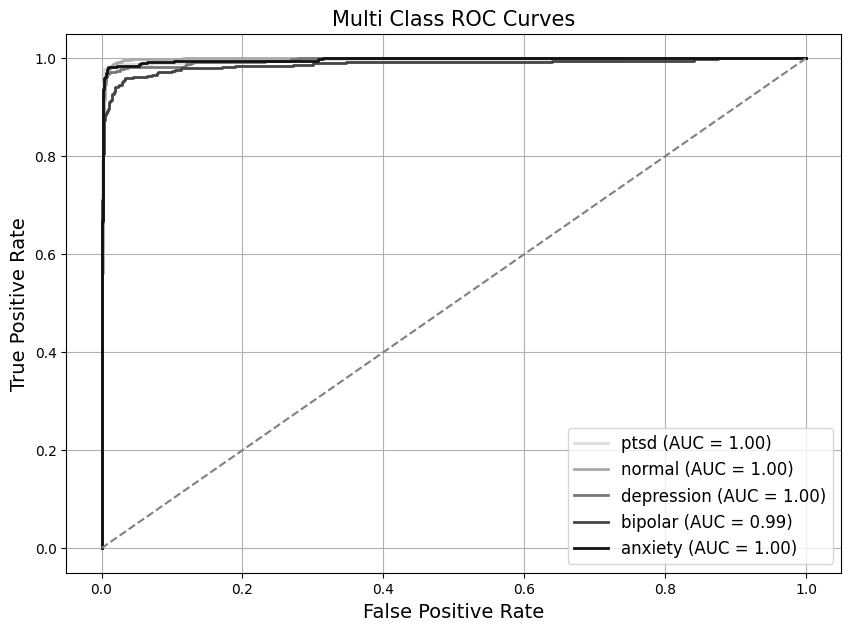
\includegraphics[width=\textwidth]{Images/BLD ROC.png}
        \caption{ROC AUC for Ensemble Model 5}
        \label{bld roc}  % Label for referencing the subfigure
    \end{subfigure}
    \caption{Evaluation Results for Ensemble Model 5}
    \label{fig:ensemble_model5_comparison}
\end{figure}

\pagebreak

\vspace{1em}
\noindent
\textbf{Ensemble Model 6}

\begin{center}
    \textbf{Cross-Validation Accuracy Scores} \\[0.5em]
    \begin{tabular}{|c|c|}
        \hline
        \textbf{Cross-Validation Accuracy Scores} & \textbf{Value} \\ \hline
        1 & 0.9582547805009426 \\ \hline
        2 & 0.9477511446269863 \\ \hline
        3 & 0.9453272286560732 \\ \hline
        4 & 0.9464045246431457 \\ \hline
        5 & 0.9488284406140587 \\ \hline
        \textbf{Mean Validation Accuracy} & \textbf{94.93\%} \\ \hline
    \end{tabular}
\end{center}

\begin{center}
    \textbf{Classification Report for Ensemble Model6} \\[0.5em]
    \begin{tabular}{|c|c|c|c|c|}
        \hline
        & \textbf{Precision} & \textbf{Recall} & \textbf{F1-Score} & \textbf{Support} \\ \hline
        \textbf{Anxiety}    & 0.95 & 0.92 & 0.94 & 400 \\ \hline
        \textbf{Bipolar}    & 0.96 & 0.74 & 0.84 & 388 \\ \hline
        \textbf{Depression} & 0.92 & 0.94 & 0.93 & 392 \\ \hline
        \textbf{Normal}     & 0.95 & 1.00 & 0.97 & 2136 \\ \hline
        \textbf{PTSD}       & 0.98 & 0.93 & 0.96 & 397 \\ \hline
        \textbf{Accuracy}   & \multicolumn{4}{c|}{\textbf{95.15\%}} \\ \hline
        \textbf{Macro avg}  & 0.95 & 0.91 & 0.93 & 3713 \\ \hline
        \textbf{Weighted avg} & 0.95 & 0.95 & 0.95 & 3713 \\ \hline
    \end{tabular}
\end{center}

\begin{figure}[h!]
    \centering
    \begin{subfigure}[b]{0.49\textwidth}
        \centering
        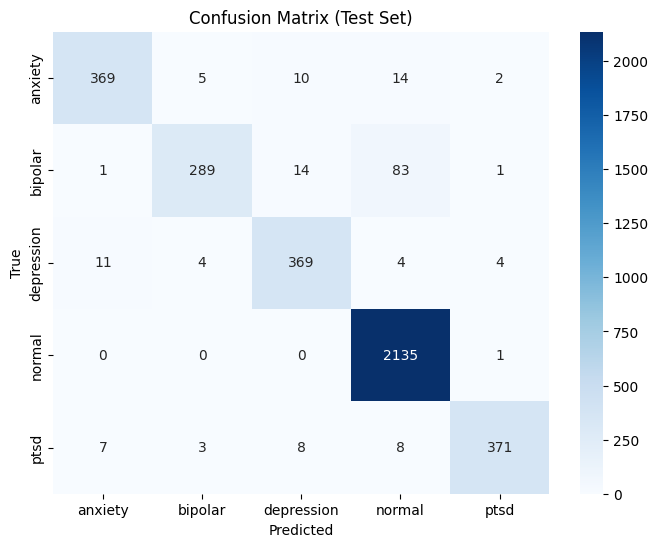
\includegraphics[width=\textwidth]{Images/WV CM.png}
        \caption{Confusion Matrix for Ensemble Model 6}
        \label{wv cm}  % Label for referencing the subfigure
    \end{subfigure}
    \hfill
    \begin{subfigure}[b]{0.49\textwidth}
        \centering
        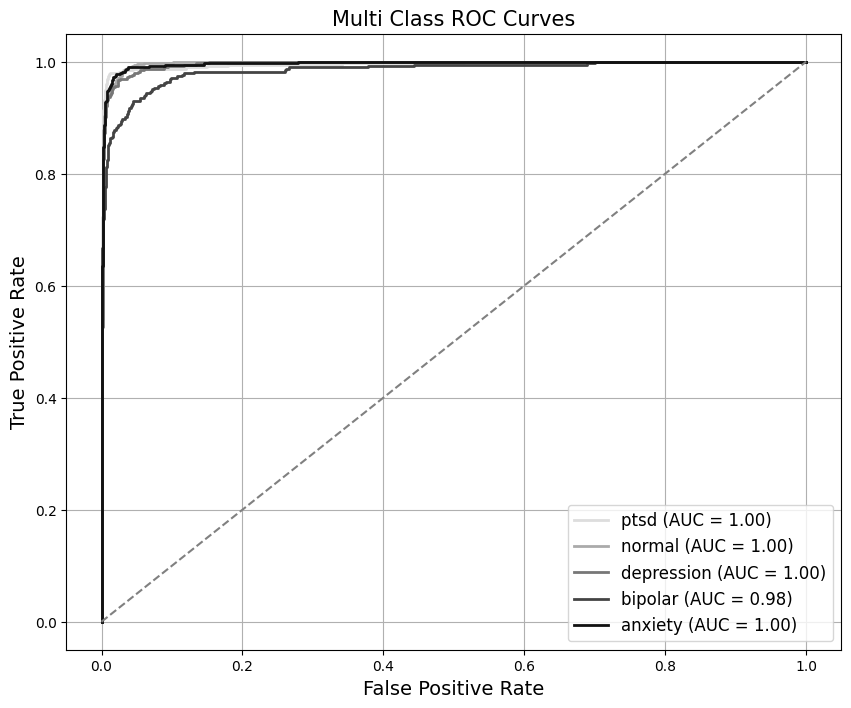
\includegraphics[width=\textwidth]{Images/WV ROC.png}
        \caption{ROC AUC for Ensemble Model 6}
        \label{wv roc}  % Label for referencing the subfigure
    \end{subfigure}
    \caption{Evaluation Results for Ensemble Model 6}
    \label{fig:ensemble_model6_comparison}
\end{figure}

\pagebreak

\vspace{1em}
\noindent
\textbf{Ensemble Model 7}

\begin{center}
    \textbf{Cross-Validation Accuracy Scores} \\[0.5em]
    \begin{tabular}{|c|c|}
        \hline
        \textbf{Cross-Validation Accuracy Scores} & \textbf{Value} \\ \hline
        1 & 0.980878 \\ \hline
        2 & 0.97899273 \\ \hline
        3 & 0.98410988 \\ \hline
        4 & 0.98168597 \\ \hline
        5 & 0.97764611 \\ \hline
        \textbf{Mean Validation Accuracy} & \textbf{98.03\%} \\ \hline
    \end{tabular}
\end{center}

\begin{center}
    \textbf{Classification Report for Ensemble Model7} \\[0.5em]
    \begin{tabular}{|c|c|c|c|c|}
        \hline
        & \textbf{Precision} & \textbf{Recall} & \textbf{F1-Score} & \textbf{Support} \\ \hline
        \textbf{Anxiety}    & 0.98 & 0.97 & 0.98 & 400 \\ \hline
        \textbf{Bipolar}    & 0.96 & 0.93 & 0.95 & 388 \\ \hline
        \textbf{Depression} & 0.97 & 0.97 & 0.97 & 392 \\ \hline
        \textbf{Normal}     & 0.99 & 1.00 & 0.99 & 2136 \\ \hline
        \textbf{PTSD}       & 0.98 & 0.98 & 0.98 & 397 \\ \hline
        \textbf{Accuracy}   & \multicolumn{4}{c|}{\textbf{98.20\%}} \\ \hline
        \textbf{Macro avg}  & 0.98 & 0.97 & 0.97 & 3713 \\ \hline
        \textbf{Weighted avg} & 0.98 & 0.98 & 0.98 & 3713 \\ \hline
    \end{tabular}
\end{center}

\begin{figure}[h!]
    \centering
    \begin{subfigure}[b]{0.49\textwidth}
        \centering
        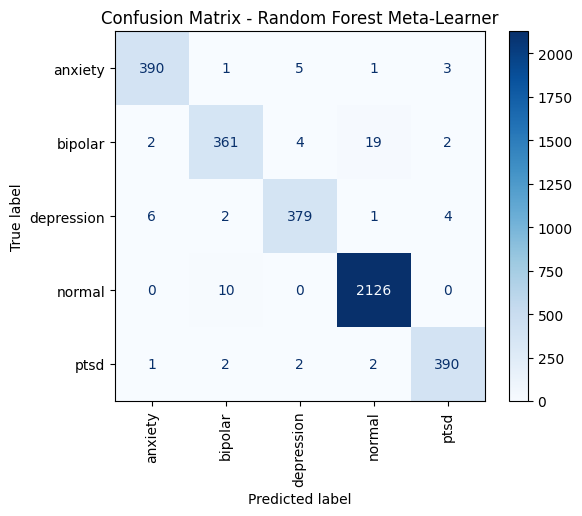
\includegraphics[width=\textwidth]{Images/EM T CM.png}
        \caption{Confusion Matrix for Ensemble Model 7}
        \label{em_t cm}  % Label for referencing the subfigure
    \end{subfigure}
    \hfill
    \begin{subfigure}[b]{0.49\textwidth}
        \centering
        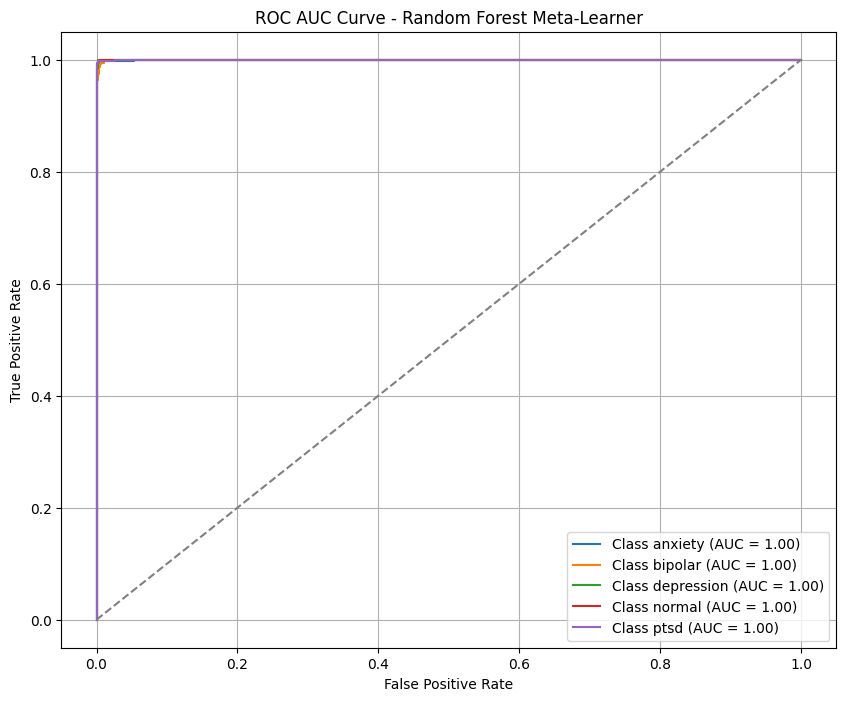
\includegraphics[width=\textwidth]{Images/EM T ROC.png}
        \caption{ROC AUC for Ensemble Model 7}
        \label{em_t roc}  % Label for referencing the subfigure
    \end{subfigure}
    \caption{Evaluation Results for Ensemble Model 7}
    \label{fig:ensemble_model7_comparison}
\end{figure}

\pagebreak

\begin{table}[H]
    \centering
    \caption*{Comparison of Ensemble Models for Mental Health Classification}
    \label{tab:ensemble_comparison}
    \begin{tabularx}{\textwidth}{|l|c|X|X|X|}
    \hline
    \textbf{Model} & \textbf{Accuracy} & \textbf{Key Components} & \textbf{Advantages} & \textbf{Limitations} \\
    \hline
    Ensemble Model 1 & 96.08\% & Logistic Regression + XGBoost & High precision and balanced performance (e.g., Anxiety: Prec=0.97, Rec=0.94, F1=0.95); robust macro/weighted averages & May not fully capture complex, non-linear, context-dependent patterns \\
    \hline
    Ensemble Model 2 & 97.93 & XGBoost as meta-learner combining base models (LR, SVM, NB, LSTM) & Near-perfect ROC AUC (1.0 for Anxiety, Normal, PTSD; 0.99 for Bipolar, Depression); effective handling of imbalanced data & Potential overfitting if base model predictions are highly correlated \\
    \hline
    Ensemble Model 3 & 97.76 & Random Forest used as meta-learner & High overall accuracy with very few misclassifications; robust due to bootstrapping and random feature selection & Slightly lower recall in some classes (e.g., Bipolar) \\
    \hline
    Ensemble Model 4 & 97.63\% & Bagging classifier (similar to Random Forest) & Excellent performance with near-perfect results for the “Normal” class & Tendency to overfit due to using all features without feature-level randomness \\
    \hline
    Ensemble Model 5 & 97.17\% & Blending Meta-Learner trained directly on base model predictions & Strong precision, recall, and F1-scores across classes; stable cross-validation performance & More prone to overfitting compared to stacking ensembles (e.g., with a Random Forest meta-learner) \\
    \hline
    Ensemble Model 6 & 95.15\% & Weighted Voting ensemble combining base model outputs & Solid overall performance with high recall for “Normal” and computational efficiency & Lacks optimal inter-model learning; struggles with distinguishing bipolar disorder \\
    \hline
\end{tabularx}
\end{table}

\begin{table}[H]
    \centering
    \caption*{Comparison of Ensemble Models for Mental Health Classification}
    \label{tab:ensemble_comparison}
    \begin{tabularx}{\textwidth}{|l|c|X|X|X|}
    \hline
    \textbf{Model} & \textbf{Accuracy} & \textbf{Key Components} & \textbf{Advantages} & \textbf{Limitations} \\
    \hline
    Ensemble Model 7 & 98.03\% & Transformer-based model (base) + meta-learner (Random Forest and others) & Near-perfect ROC AUC (1.0 across classes); excellent accuracy and robust classification & Increased computational complexity due to Transformer integration \\
    \hline
    \end{tabularx}
\end{table}

    
\begin{figure}[h!]  
    \centering
    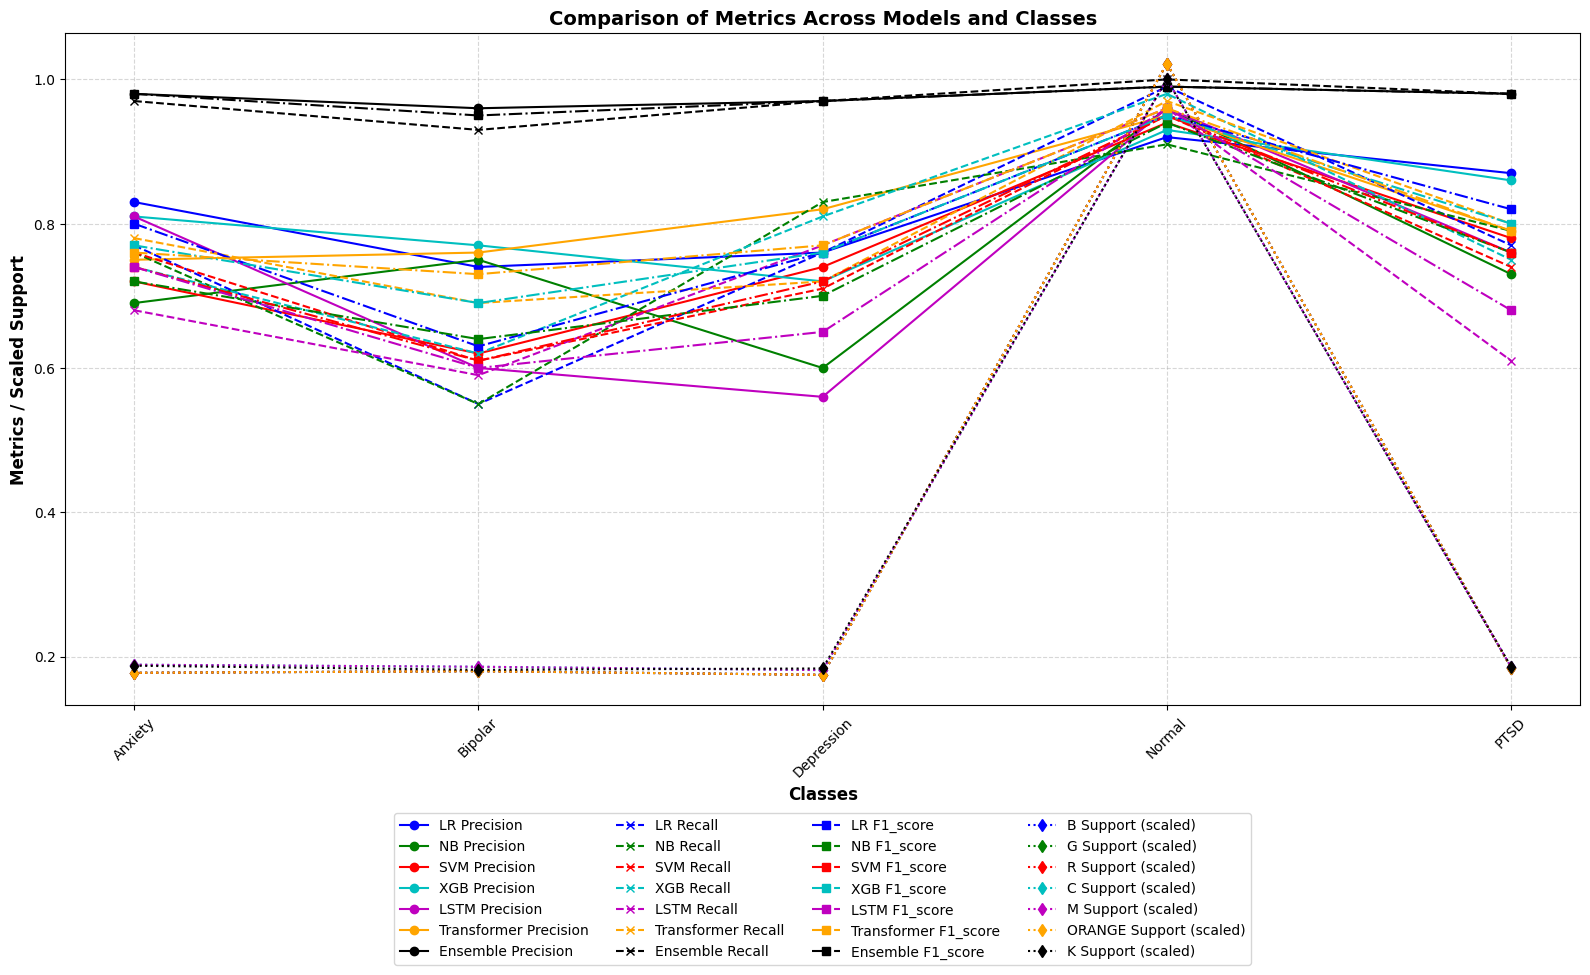
\includegraphics[width=1.0\textwidth]{Images/EM T RESULT.png}  
    \caption{Comparison of Base Models and Ensemble Model7}
    \label{lstm arch}  % Label for referencing the figure
\end{figure}

\pagebreak

\noindent
Below is a comparison of all the ensemble models for reference

\begin{figure}[h!]  
    \centering
    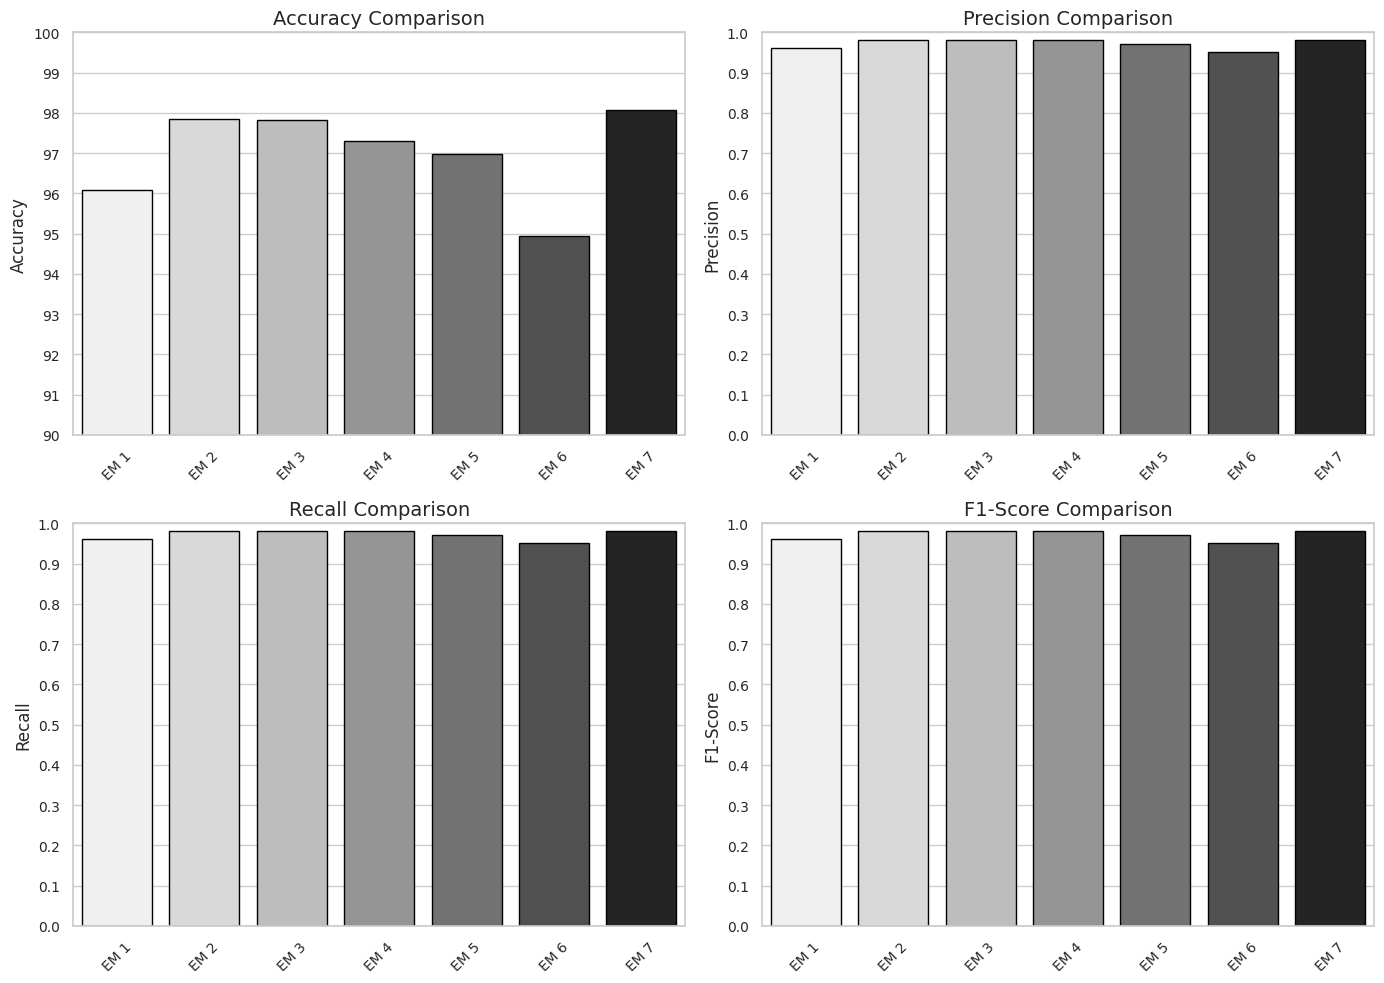
\includegraphics[width=1.0\textwidth]{Images/EM COMPARE.png}  
    \caption{Comparison of all Ensemble Models}
    \label{lstm arch}  % Label for referencing the figure
\end{figure}



\subsection{Result from hierarchical Ensemble Models}

\noindent
Ensemble Model 7 is applied on different subsets of a very large dataset to create hierarchical ensemble models. The performance of each model is evaluated, and the results are compared to the global ensemble model. 

\begin{center}
    \textbf{Performance Comparison of Models} \\[0.5em]
    % Resize the table to fit the text width
    \resizebox{\textwidth}{!}{%
    \begin{tabular}{|c|c|c|c|c|c|c|c|}
        \hline
        \textbf{Model} & \textbf{Subset 1} & \textbf{Subset 2} & \textbf{Subset 3} & \textbf{Subset 4} & \textbf{Subset 5} & \textbf{Subset 6} & \textbf{ENSEMBLE} \\ \hline
        Logistic Regression & 87.66 & 85.07 & 86.74 & 90.61 & 88.17 & 72.62 & \textbf{90.90} \\ \hline
        Naive Bayes         & 83.63 & 81.71 & 83.50 & 84.44 & 85.93 & 64.33 & \textbf{84.15} \\ \hline
        SVM                 & 85.13 & 82.30 & 83.50 & 88.34 & 85.45 & 67.81 & \textbf{91.79} \\ \hline
        XGBoost             & 87.39 & 85.79 & 86.78 & 91.37 & 86.32 & 70.95 & \textbf{67.67} \\ \hline
        LSTM                & 84.91 & 81.63 & 81.83 & 87.22 & 85.38 & 67.74 & \textbf{87.48} \\ \hline
        Transformer         & 88.50 & 84.50 & 86.50 & 89.35 & 87.62 & 72.40 & \textbf{91.53} \\ \hline
        \textbf{ENSEMBLE}   & \textbf{98.03} & \textbf{94.85} & \textbf{96.96} & \textbf{97.79} & \textbf{96.86} & \textbf{92.57} & 
        \diagbox[height=2em,width=7em]%
        {\makebox[2.5em][r]{\textbf{96.24}}}%
        {\makebox[2.5em][l]{\textbf{96.25}}} \\ \hline
    \end{tabular}
    } % End of resizebox
    \\[1em]
    \textbf{Note:} The final ensemble models from two different architectures achieved accuracies of \textbf{96.24\%} and \textbf{96.25\%} respectively.
\end{center}

\noindent
The hierarchical ensemble model addresses the challenge of handling large datasets by adopting a modular and scalable approach. The dataset is divided into manageable subsets, each treated independently. For each subset, base models like Logistic Regression, Naive Bayes, SVM, LSTM, XGBoost, and Custom Transformers are trained and combined into a subset-specific ensemble using Random Forest as the meta learner. These subset ensembles are then aggregated to form a final global ensemble, capturing comprehensive learning from the entire dataset. This approach ensures efficient handling of large-scale data while maintaining high performance. Although the current implementation is sequential for testing purposes, the design is inherently scalable to a distributed architecture. In such a setup, subsets can be processed in parallel across multiple computational nodes. Each node trains base models, creates a subset ensemble, and sends results to a central controller, which aggregates them into a global ensemble. This parallelized framework aligns with distributed computing principles, making it ideal for real-world, large-scale applications. 

\vspace{1em}

\noindent
The hierarchical structure of this approach aligns with distributed systems by effectively implementing data parallelism and task parallelism. By dividing the dataset into subsets, the computational load is distributed, preventing memory bottlenecks and ensuring resource optimization. Each subset is processed independently, enabling a modular design where tasks are decoupled. This design also enhances fault tolerance, as the failure of a single subset’s processing does not affect the others. Moreover, the scalability of the approach allows it to adapt to varying resource constraints. Adding more computational nodes makes it feasible to handle additional subsets or process the data faster, showcasing its adaptability and efficiency. The distributed nature of the architecture ensures high throughput and reduces training time, making it suitable for scenarios involving large-scale datasets. The hierarchical ensemble model design is a future-ready solution that can transition seamlessly to distributed platforms, leveraging cloud services or on-premises high-performance computing clusters. The methodology combines the strengths of ensemble learning with the efficiencies of distributed systems to create a robust and scalable solution for modern data science challenges.

\vspace{1em}

\begin{figure}[h!]  
    \centering
    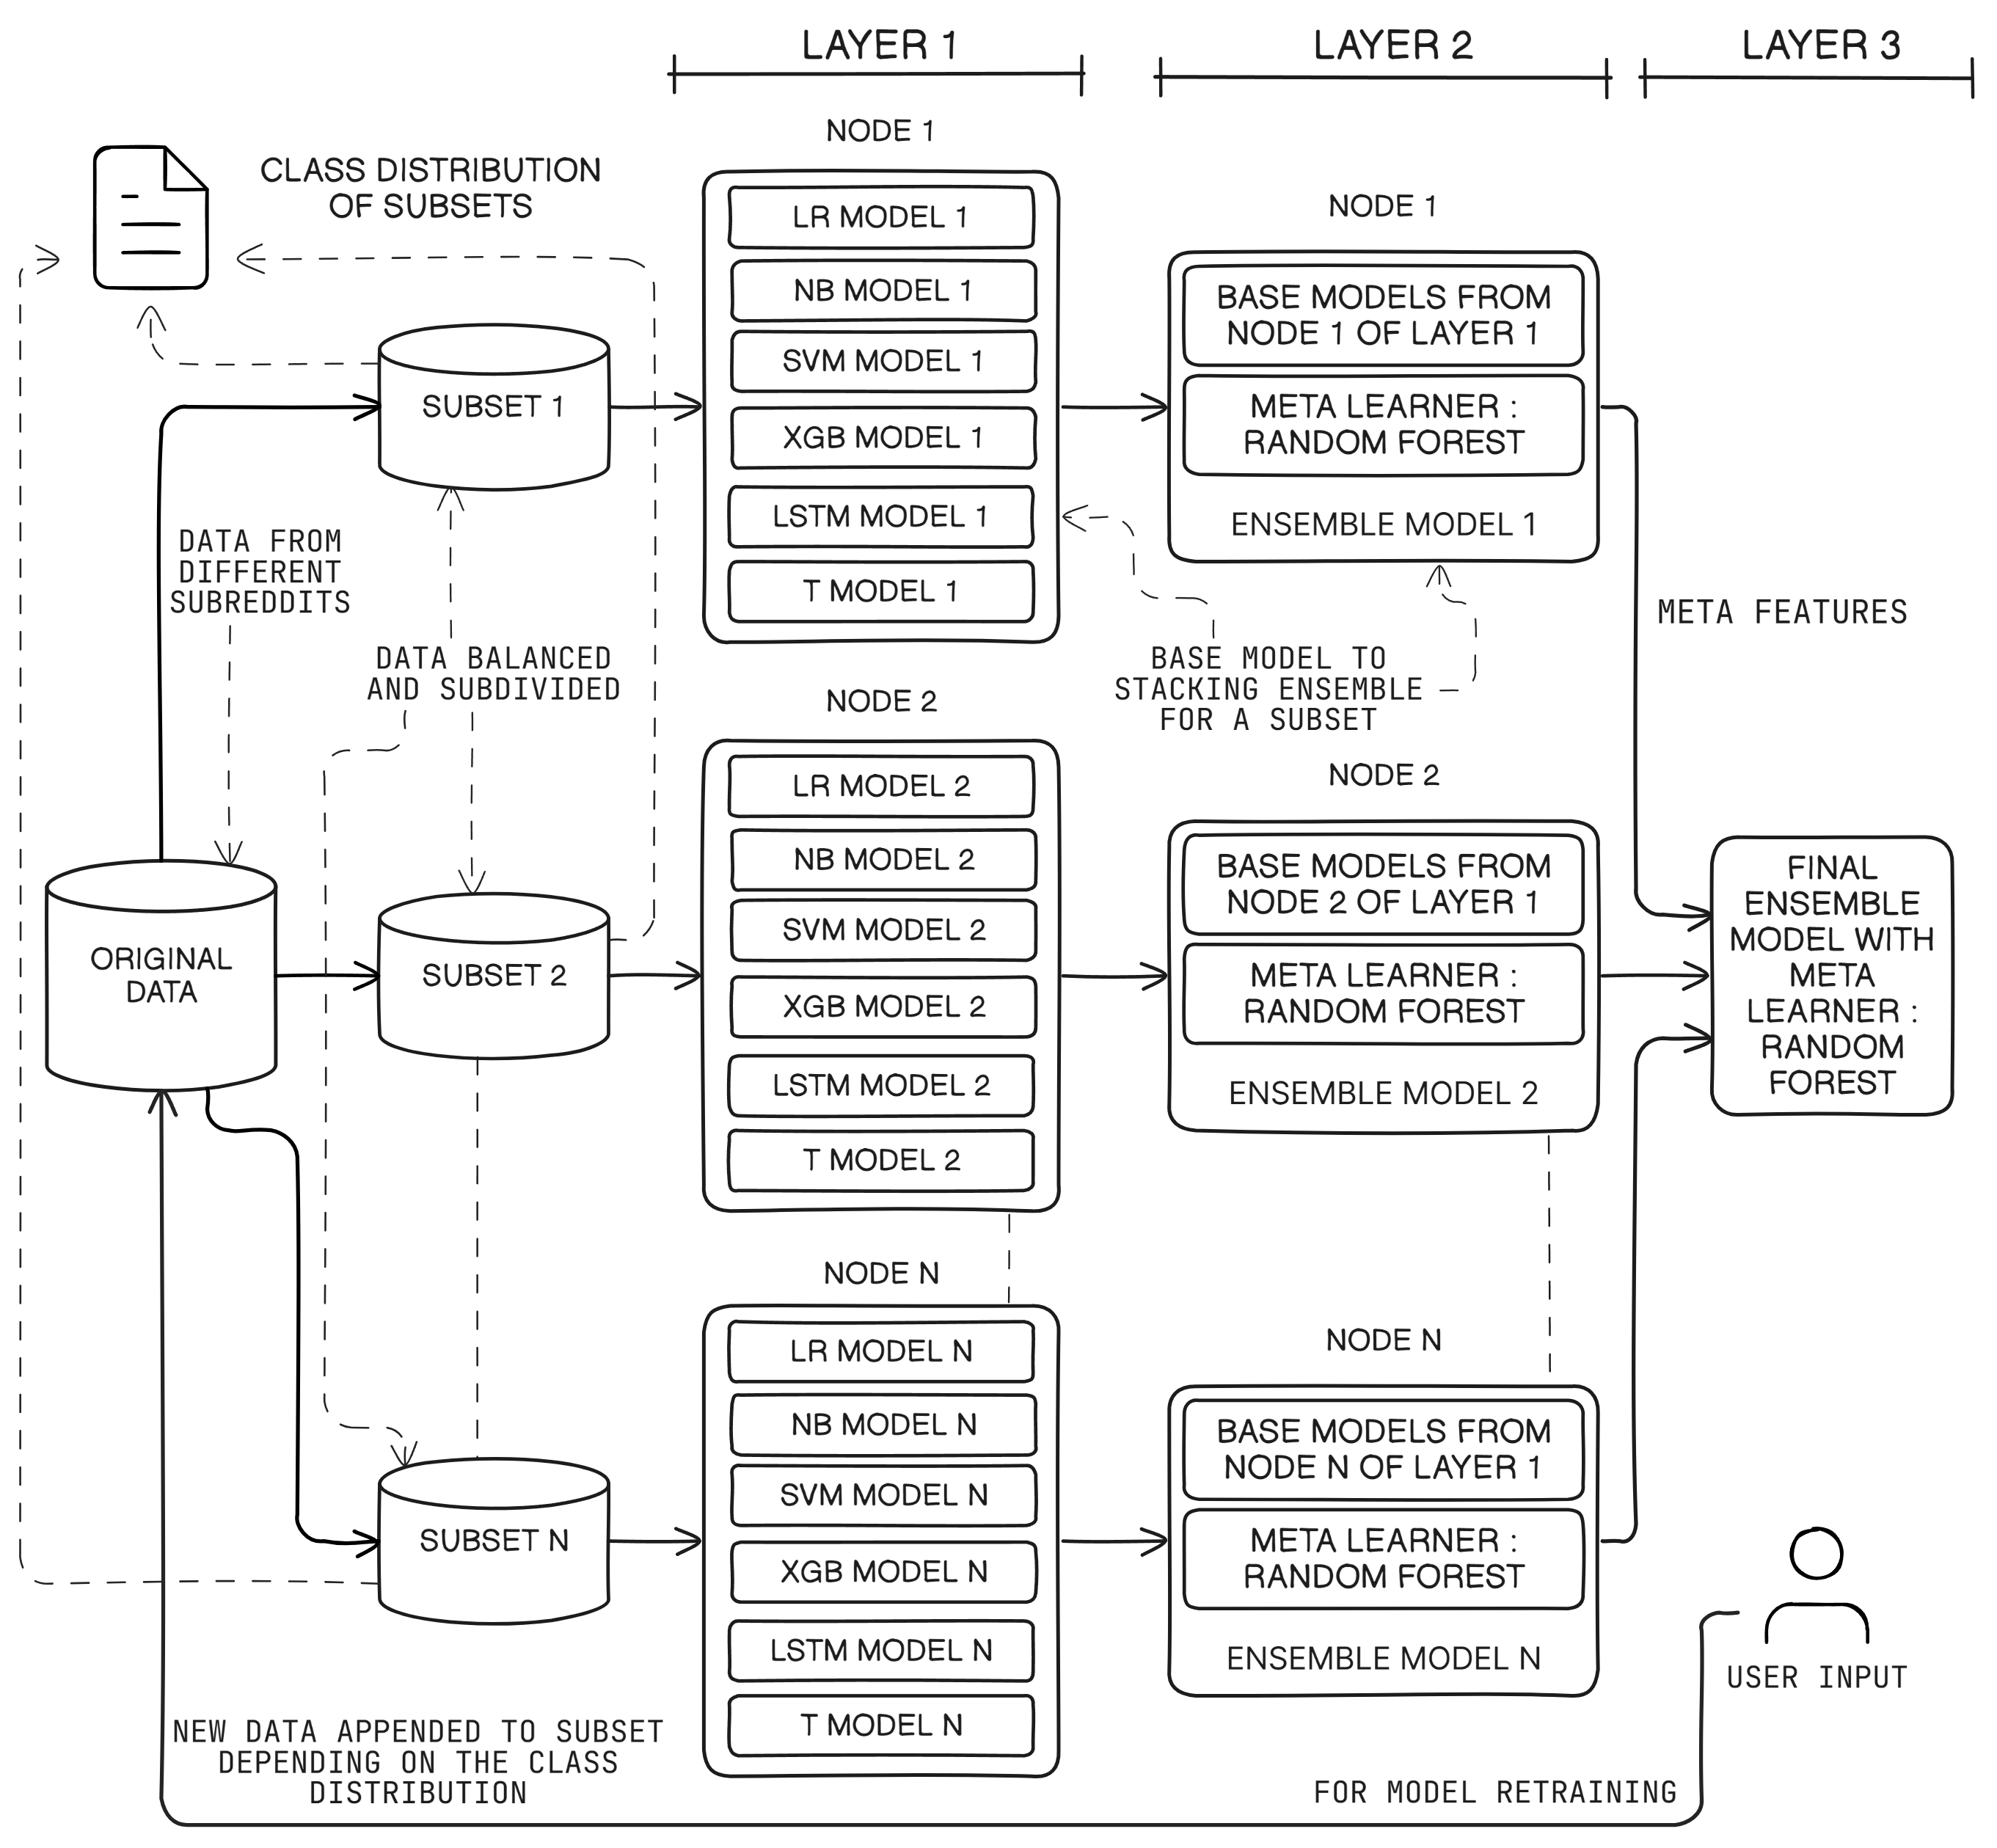
\includegraphics[width=1.0\textwidth]{Images/Distributed.png}  
    \caption{Scalable Distributed Architecture 1}
    \label{lstm archi}  % Label for referencing the figure
\end{figure}


\begin{figure}[h!]  
    \centering
    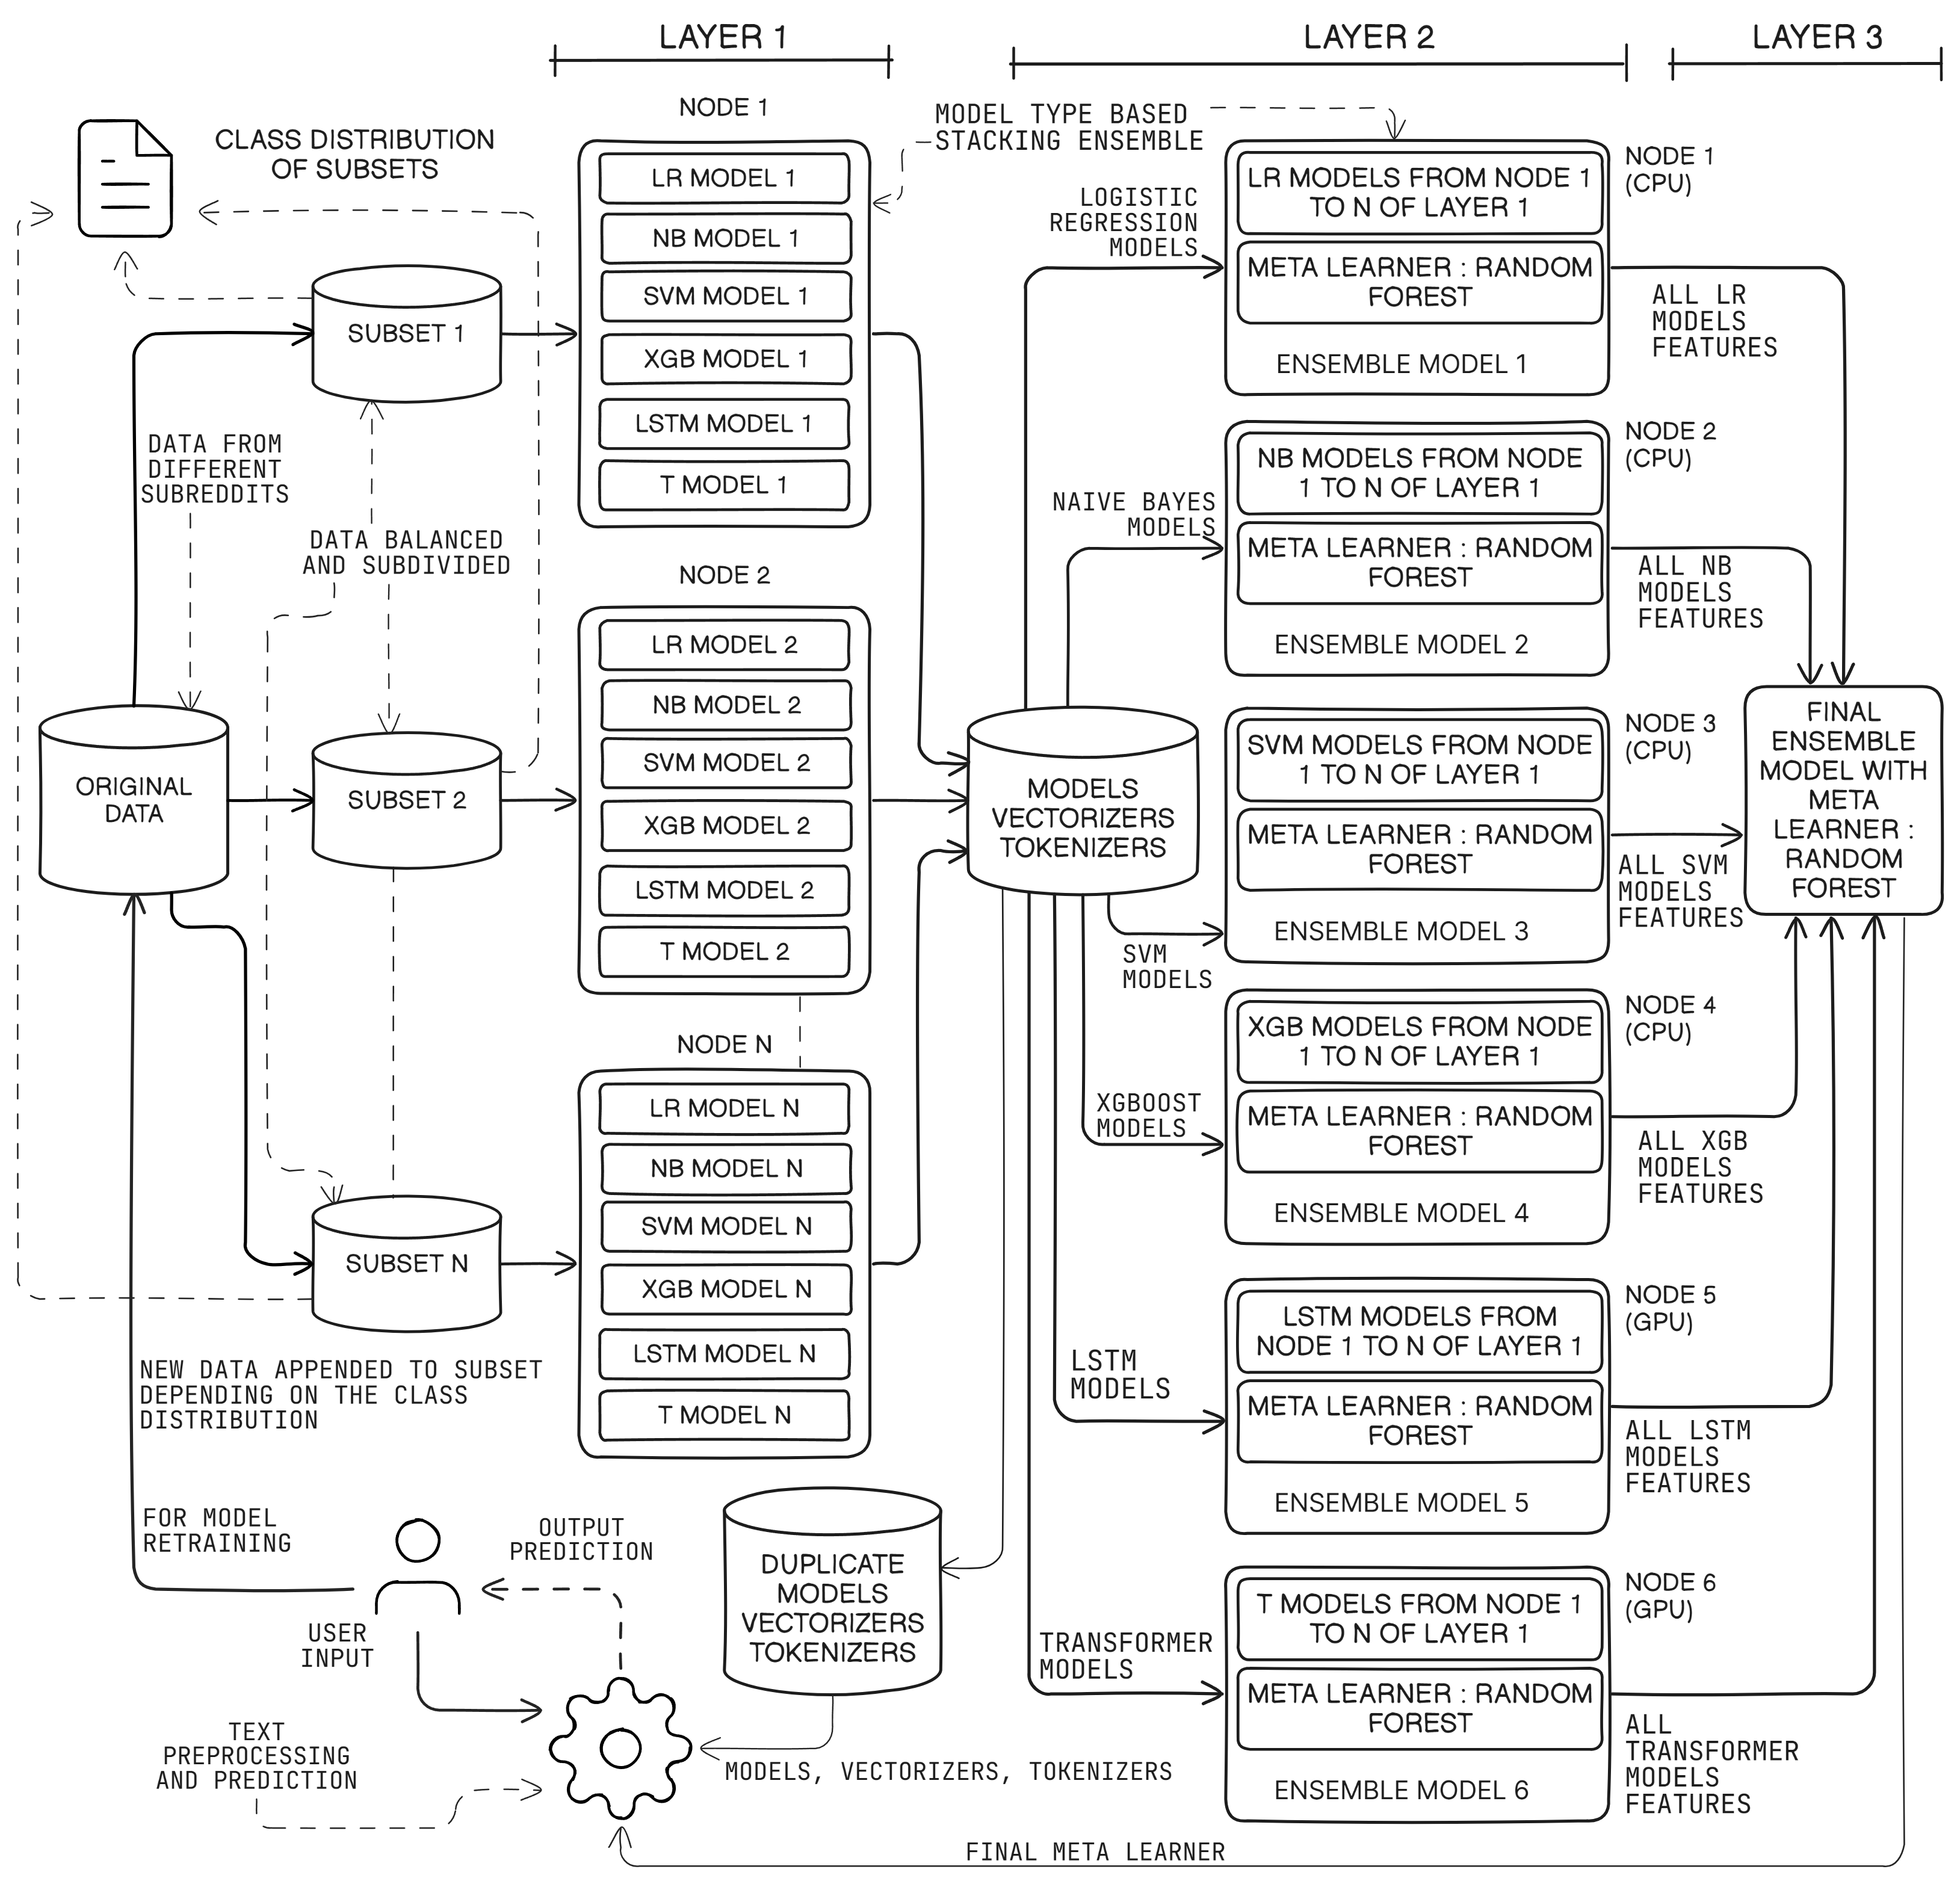
\includegraphics[width=1.0\textwidth]{Images/Distributed2.png}  
    \caption{Scalable Distributed Architecture 2}
    \label{lstm archi}  % Label for referencing the figure
\end{figure}


\noindent
The second architecture optimizes the hierarchical ensemble approach by restructuring the model aggregation process to enhance scalability and computational efficiency. Instead of creating ensemble models for each of the $n$ subsets independently, models of the same type from all subsets are combined into a single ensemble for that type using Random Forest (or Logistic Regression) as the meta learner. This results in six intermediate ensemble models, one for each model type: Logistic Regression, Naive Bayes, SVM, XGBoost, LSTM, and Transformer. These intermediate ensemble models are then used to form the final ensemble model, where Random Forest acts as the meta learner. This architectural adjustment significantly reduces the number of intermediate ensemble models from $n$ to six while preserving the hierarchical structure, thereby maintaining a consistent three-layer design. The second architecture achieved an accuracy of 96.25\%. However, its design provides distinct advantages when dealing with much larger datasets or a higher number of subsets. As the dataset size increases, the number of subsets and computational nodes may also grow. In the previous architecture, this scaling would lead to a proportional increase in the number of intermediate ensemble models, which could strain computational resources and introduce inefficiencies in model aggregation. In contrast, the second architecture fixes the number of intermediate ensemble models at six, irrespective of the number of subsets, ensuring that the computational load remains manageable while scalability is maintained. Another significant improvement lies in the efficient use of hardware resources. In the second architecture, GPUs are utilized exclusively for training the LSTM and Transformer-based ensemble models, rather than being partially engaged across all intermediate models as in the first architecture. This selective usage of GPUs streamlines resource allocation, ensuring that the most computationally intensive models benefit from accelerated hardware while reducing unnecessary overhead for other model types. The use of Logistic Regression as the meta learner in the intermediate ensemble models further contributes to this efficiency. Logistic Regression is computationally lightweight and linear, making it an excellent choice for aggregating predictions across subsets without introducing excessive complexity. Its linearity ensures faster training while maintaining strong predictive performance, particularly for well-separated data classes. Random Forest as a meta-learner is a better option for considering overfitting issues. A key addition to the second architecture is the implementation of an efficient data bus for transferring models of the same type from different subsets to the respective intermediate nodes responsible for creating the type-specific ensemble. This structured flow of data and models ensures seamless communication between subsets and intermediate nodes, reducing latency and synchronization overhead. By fixing the number of intermediate ensemble models at six, the architecture limits the number of aggregation layers while still leveraging the diversity and complementary strengths of all base models. This design strikes a balance between computational efficiency and predictive performance, making it particularly advantageous for large-scale datasets. The second architecture's streamlined design, efficient resource utilization, and fixed number of intermediate ensemble models make it a robust and scalable solution for modern data science challenges. By addressing the potential bottlenecks of the first architecture while maintaining comparable performance, it provides a practical alternative for real-world applications where scalability and computational efficiency are critical.

\vspace{1em}

\noindent
Architecture 1 takes more time in cross-validation compared to Architecture 2 due to its decentralized design. In Architecture 1, each subset independently creates its intermediate ensemble model, resulting in a larger number of models being trained and validated. This increases the computational workload and requires more synchronization across subsets. On the other hand, Architecture 2 aggregates models of the same type into a single intermediate ensemble model, reducing the number of intermediate ensembles. This streamlining minimizes redundancy and allows for faster cross-validation while maintaining predictive performance. In Architecture 2, models of the same type are used as base models in the intermediate ensemble to ensure consistency and simplify the aggregation process. Mixing different types of models, such as Logistic Regression from one subset and SVM from another, would introduce heterogeneity in predictions, making the meta-learning process more complex. By grouping models of the same type, the meta-learner can better capture specific patterns and variations unique to each model type. This design also ensures that the strengths of each algorithm are utilized optimally, allowing the final ensemble to benefit from their complementary capabilities. The observation that SMOTE is not required and yields the same results as stratified K-fold cross-validation indicates that the dataset is either balanced or sufficiently robust to handle minor class imbalances. Stratified K-fold cross-validation ensures that each fold maintains the same class distribution as the original dataset, effectively mitigating the impact of class imbalance during training and testing. This suggests that the dataset's inherent balance, combined with the model’s robustness, eliminates the need for synthetic oversampling techniques like SMOTE. Logistic Regression with L1 or L2 regularization is less suited for Architecture 2 because it takes more time to train on the larger, aggregated datasets at the intermediate level. Regularization adds computational overhead by optimizing penalty terms alongside the model's weights, which can slow down training. Furthermore, Logistic Regression may struggle with the diverse, high-dimensional feature space created by aggregated predictions from multiple subsets. Random Forest, as a meta-learner, is a better choice in Architecture 2 because it is less prone to overfitting, can capture nonlinear relationships, and handles high-dimensional data effectively without extensive parameter tuning. Its ensemble-based nature ensures better generalization, making it more efficient and reliable for intermediate and final aggregation.

\vspace{1em}

\noindent
To determine \( n \), the number of subsets, based on the size of the original dataset, it is crucial to consider computational efficiency, memory constraints, and sequential execution. Given that the dataset has \( D = 167,229 \) records and is processed sequentially in Google Colab with 12GB of RAM per node, the number of subsets \( n \) must strike a balance between memory usage and model performance. In this case, you chose \( n = 6 \) subsets, which implies a subset size \( S \) of:

\[
S = \frac{D}{n} = \frac{167,229}{6} \approx 27,872 \, \text{records per subset}.
\]

\vspace{1em}

\noindent
The choice of \( n = 6 \) is reasonable given the following factors:

\vspace{1em}

\noindent
1. \textbf{Memory Constraints}: Google Colab provides 12GB of RAM. Each subset must fit within this memory while accommodating the model's requirements for training and validation. Processing approximately 27,833 records at a time is well-suited to this memory limit for most machine learning models, including Logistic Regression, SVM, LSTM, and Transformer-based models.

\noindent
2. \textbf{Sequential Execution}: Since the architectures are implemented sequentially, the number of subsets \( n \) does not need to align with the number of computational nodes. Instead, the goal is to divide the dataset into manageable chunks that reduce training time and memory overhead for each subset.

\noindent
3. \textbf{Performance and Aggregation}: With \( n = 6 \), both architectures remain computationally feasible. In Architecture 1, \( n = 6 \) leads to six independent intermediate ensemble models, which are aggregated into the final ensemble. In Architecture 2, models of the same type from all six subsets are combined into six intermediate ensemble models, one for each type of algorithm.

\vspace{1em}

\noindent
The web application does not use the model for bigger dataset but focuses on the model received from the first intermediate node of Architecture 1. The reason being that the model for the bigger dataset takes a lot of time, more than 20 minutes, if the user chooses for retraining the model after an input.

\pagebreak

% ------------------------ Result and Analysis Ends -------------------------
